% ============================================================
% BTL MAD 2026 - Phase 1: Phần Chung, Mô Tả Và Đặc Tả Đề Tài
% Ứng dụng: Pody
% ============================================================
\documentclass[14pt,a4paper,oneside]{extreport}

% ---- Encoding & Font ----
\usepackage[utf8]{inputenc}
\usepackage[T5]{fontenc}
\usepackage[vietnamese]{babel}
\usepackage{times}              % Times New Roman

% ---- Geometry ----
\usepackage[
  top=2.5cm,
  bottom=2.5cm,
  left=3cm,
  right=2cm
]{geometry}

% ---- Packages ----
\usepackage{graphicx}
\usepackage{float}
\usepackage{array}
\usepackage{booktabs}
\usepackage{longtable}
\usepackage{tabularx}
\usepackage{enumitem}
\usepackage{hyperref}
\usepackage{xcolor}
\usepackage{fancyhdr}
\usepackage{titlesec}
\usepackage{caption}
\usepackage{indentfirst}
\usepackage{setspace}
\usepackage{listings}
\usepackage{tikz}

\newcommand{\coverpageborder}{%
  \begin{tikzpicture}[remember picture,overlay]
    \draw[line width=1.2pt]
      ([xshift=1.5cm,yshift=-1.5cm]current page.north west)
      rectangle
      ([xshift=-1.5cm,yshift=1.5cm]current page.south east);
    \draw[line width=0.4pt]
      ([xshift=1.65cm,yshift=-1.65cm]current page.north west)
      rectangle
      ([xshift=-1.65cm,yshift=1.65cm]current page.south east);
  \end{tikzpicture}%
}

% ---- Hyperref setup ----
\hypersetup{
  colorlinks=true,
  linkcolor=black,
  citecolor=black,
  urlcolor=blue
}

% ---- Spacing ----
\onehalfspacing
\setlength{\parindent}{1cm}

% ---- Header/Footer ----
\pagestyle{fancy}
\fancyhf{}
\fancyfoot[C]{\thepage}
\renewcommand{\headrulewidth}{0pt}

% ---- Chapter/Section Format ----
\titleformat{\chapter}[display]
  {\normalfont\Large\bfseries\centering}
  {\MakeUppercase{\chaptertitlename}\ \thechapter}{10pt}{\Large\MakeUppercase}
\titlespacing*{\chapter}{0pt}{-20pt}{20pt}

\titleformat{\section}
  {\normalfont\large\bfseries}{\thesection}{1em}{}
\titleformat{\subsection}
  {\normalfont\normalsize\bfseries}{\thesubsection}{1em}{}

% ---- Captions ----
\captionsetup{font=small, labelfont=bf}

% ---- List of Tables/Figures naming ----
\renewcommand{\listtablename}{Danh sách bảng biểu}
\renewcommand{\listfigurename}{Danh sách hình vẽ}
\renewcommand{\contentsname}{Mục lục}
\renewcommand{\chaptername}{Chương}
\renewcommand{\tablename}{Bảng}
\renewcommand{\figurename}{Hình}

% ============================================================
\begin{document}

% ============================================================
% TRANG BÌA
% ============================================================
\begin{titlepage}
  \coverpageborder
  \begin{center}

    \textbf{\large HỌC VIỆN CÔNG NGHỆ BƯU CHÍNH VIỄN THÔNG}\\[2pt]
    \textbf{\large KHOA CÔNG NGHỆ THÔNG TIN}

    \vspace{0.35cm}

    
\includegraphics[width=2.4cm]{assets/logo_ptit.png}

    \vspace{0.45cm}

    {\large\textbf{BÁO CÁO BÀI TẬP LỚN}}\\[6pt]
    {\Large\textbf{PHÁT TRIỂN ỨNG DỤNG CHO\\THIẾT BỊ DI ĐỘNG (MAD)}}

    \vspace{0.6cm}

    {\LARGE\textbf{ỨNG DỤNG PODY}}\\[6pt]
    {\large\textit{Nền tảng nghe podcast và tạo nội dung\\podcast hỗ trợ AI}}

    \vspace{0.8cm}

    \begin{tabular}{r l}
      \textbf{Giảng viên hướng dẫn:} & \textit{ThS. Nguyễn Hoàng Anh} \\[6pt]
      \textbf{Nhóm QLĐT:}           & \textit{CNPM05} \\[6pt]
      \textbf{Nhóm BTL:}             & \textit{01} \\
      \textbf{Thành viên thực hiện:} & \textit{Lê Minh Ngọc -- B22DCCN586} \\[6pt]
    \end{tabular}

    \vspace{0.45cm}

    \textbf{Danh sách thành viên:}

    \vspace{0.2cm}

    \begin{tabular}{|c|l|c|}
      \hline
      \textbf{STT} & \textbf{Họ và tên} & \textbf{MSSV} \\
      \hline
      1 & Lại Xuân Hiếu & B22DCCN309 \\
      \hline
      2 & Vũ Đức Thành & B22DCCN801 \\
      \hline
      3 & Nguyễn Việt Huy & B22DCCN393 \\
      \hline
      4 & Lê Minh Ngọc & B22DCCN586 \\
      \hline
    \end{tabular}

    \vfill

    \textbf{Hà Nội, 2026}

  \end{center}
\end{titlepage}

% ============================================================
% TRANG THÀNH VIÊN VÀ ĐÓNG GÓP
% ============================================================
\newpage
\thispagestyle{fancy}
\begin{center}
  {\Large\textbf{BẢNG PHÂN CÔNG THÀNH VIÊN VÀ ĐÓNG GÓP}}
\end{center}

\vspace{0.5cm}

\noindent
Bảng dưới đây trình bày chi tiết phân công công việc và phạm vi phụ trách của từng thành viên trong nhóm.

\vspace{0.5cm}

\begin{table}[H]
\centering
\caption{Phân công thành viên và đóng góp}
\label{tab:phan-cong}
\renewcommand{\arraystretch}{1.4}
\small
\begin{tabularx}{\textwidth}{|c|l|c|l|X|c|}
\hline
\textbf{STT} & \textbf{Họ và tên} & \textbf{MSSV} & \textbf{Vai trò} & \textbf{Phạm vi phụ trách \& Công việc} & \textbf{\%} \\
\hline
1 &
  \textit{Lại Xuân Hiếu} &
  \textit{B22DCCN309} &
  Thành viên &
  AI tạo podcast -- \texttt{ai-service}, \texttt{content-service}. Phụ trách luồng creator tạo podcast/show bằng AI, quản lý voice profiles, chat-create, production plan, job tạo show/episode, home feed, bookmark. &
  25\% \\
\hline
2 &
  \textit{Vũ Đức Thành} &
  \textit{B22DCCN801} &
  Thành viên &
  Báo và podcast báo -- \texttt{article\_service}, \texttt{embedding\_service}. Phụ trách crawl bài báo, category, tương tác bài viết, tạo podcast từ nhóm bài báo, embedding/search semantic, gán category ngữ nghĩa. &
  25\% \\
\hline
3 &
  \textit{Nguyễn Việt Huy} &
  \textit{B22DCCN393} &
  Thành viên &
  Hạ tầng và xác thực -- \texttt{api-gateway}, \texttt{identity-service}. Phụ trách cửa vào hệ thống, routing, JWT auth, đăng ký/đăng nhập, xác minh email, password reset, outbox event. &
  25\% \\
\hline
4 &
  \textit{Lê Minh Ngọc} &
  \textit{B22DCCN586} &
  Thành viên &
  Thông báo -- \texttt{notification-service}. Phụ trách notification inbox, unread count, settings, email hệ thống, consume Kafka event, retry/DLQ, delivery logs. &
  25\% \\
\hline
\end{tabularx}
\end{table}

% ============================================================
% MỤC LỤC
% ============================================================
\newpage
\tableofcontents

% ============================================================
% DANH SÁCH HÌNH VẼ
% ============================================================
\newpage
\listoffigures

% ============================================================
% DANH SÁCH BẢNG BIỂU
% ============================================================
\listoftables

% ============================================================
% DANH SÁCH TỪ VIẾT TẮT
% ============================================================
\newpage
\begin{center}
  {\Large\textbf{DANH SÁCH TỪ VIẾT TẮT}}
\end{center}

\vspace{0.5cm}

\begin{longtable}{l l}
  \toprule
  \textbf{Từ viết tắt} & \textbf{Giải thích} \\
  \midrule
  \endfirsthead

  \toprule
  \textbf{Từ viết tắt} & \textbf{Giải thích} \\
  \midrule
  \endhead

  AI    & Artificial Intelligence -- Trí tuệ nhân tạo \\
  API   & Application Programming Interface -- Giao diện lập trình ứng dụng \\
  CDC   & Change Data Capture -- Thu thập thay đổi dữ liệu \\
  CORS  & Cross-Origin Resource Sharing -- Chia sẻ tài nguyên nguồn chéo \\
  CRUD  & Create, Read, Update, Delete \\
  DB    & Database -- Cơ sở dữ liệu \\
  DLQ   & Dead Letter Queue -- Hàng đợi thư chết \\
  ER    & Entity-Relationship -- Thực thể - Quan hệ \\
  GCS   & Google Cloud Storage \\
  JWT   & JSON Web Token \\
  MAD   & Mobile Application Development -- Phát triển ứng dụng di động \\
  REST  & Representational State Transfer \\
  RSS   & Really Simple Syndication \\
  SMTP  & Simple Mail Transfer Protocol \\
  SQL   & Structured Query Language \\
  TTS   & Text-to-Speech -- Chuyển văn bản thành giọng nói \\
  UI    & User Interface -- Giao diện người dùng \\
  \bottomrule
\end{longtable}

% ============================================================
% CHƯƠNG 1 - MỞ ĐẦU VÀ YÊU CẦU
% ============================================================
\chapter{MỞ ĐẦU VÀ YÊU CẦU}
\label{chap:mo-dau}

% ---- 1.1 Giới thiệu ứng dụng ----
\section{Giới thiệu ứng dụng}
\label{sec:gioi-thieu}

\textbf{Pody} là một nền tảng ứng dụng di động cho phép người dùng nghe podcast, đọc bài báo và tạo nội dung podcast với sự hỗ trợ của trí tuệ nhân tạo (AI). Ứng dụng được thiết kế để phục vụ hai nhóm người dùng chính:

\begin{itemize}[leftmargin=2cm]
  \item \textbf{Listener (Người nghe):} Có thể đăng ký/đăng nhập tài khoản, khám phá nội dung trên trang chủ, đọc và tìm kiếm bài báo theo category hoặc tìm kiếm ngữ nghĩa (semantic search), nghe podcast, lưu tập yêu thích (bookmark), tương tác với bài viết thông qua reaction/comment và theo dõi thông báo trong ứng dụng.

  \item \textbf{Creator (Nhà sáng tạo nội dung):} Có thể sử dụng AI để trò chuyện, lên kế hoạch sản xuất (production plan), tạo show và episode podcast một cách tự động. Creator cũng có thể chọn nhóm bài báo để tạo podcast dạng tổng hợp tin tức.
\end{itemize}

Hệ thống Pody được xây dựng theo kiến trúc \textbf{microservices}, bao gồm ứng dụng Flutter cho phía client, một API Gateway điều phối và xác thực, cùng nhiều backend service độc lập phụ trách các nghiệp vụ riêng biệt. Mỗi service có cơ sở dữ liệu riêng, giao tiếp qua REST API và sự kiện bất đồng bộ qua Apache Kafka.

% ---- 1.2 Lý do chọn đề tài ----
\section{Lý do chọn đề tài}
\label{sec:ly-do}

Việc lựa chọn đề tài Pody xuất phát từ các lý do sau:

\begin{enumerate}[leftmargin=2cm]
  \item \textbf{Xu hướng tiêu thụ nội dung dạng âm thanh:} Nhu cầu nghe podcast và tiêu thụ nội dung ngắn dạng âm thanh đang tăng trưởng mạnh mẽ trên toàn cầu. Người dùng ngày càng ưa chuộng việc nghe nội dung trong lúc di chuyển, tập thể dục hay làm việc nhà thay vì đọc bài viết dài.

  \item \textbf{Nhu cầu tóm tắt và chuyển đổi nội dung:} Tin tức và nội dung dài cần được tóm tắt, chuyển đổi thành dạng dễ nghe hơn. Podcast là phương tiện phù hợp để truyền tải thông tin một cách ngắn gọn và sinh động.

  \item \textbf{AI hỗ trợ sáng tạo nội dung:} Trí tuệ nhân tạo có thể hỗ trợ lập kế hoạch sản xuất, tạo kịch bản (script), tạo transcript và audio thông qua TTS (Text-to-Speech), giúp rút ngắn đáng kể thời gian sản xuất podcast so với quy trình truyền thống.

  \item \textbf{Phù hợp để áp dụng nhiều công nghệ hiện đại:} Đề tài là môi trường lý tưởng để áp dụng đồng thời nhiều công nghệ: mobile app (Flutter), backend microservices (Go, Python/FastAPI), AI/ML (Google GenAI, embedding, TTS), tìm kiếm ngữ nghĩa (pgvector), kiến trúc event-driven (Kafka, Debezium), hệ thống thông báo và nhiều hơn nữa.
\end{enumerate}

% ---- 1.3 Concept thực hiện ứng dụng ----
\section{Concept thực hiện ứng dụng}
\label{sec:concept}

Concept cốt lõi của Pody được tóm gọn trong câu:

\begin{center}
  \textit{\textbf{``Đọc nhanh, nghe sau, tạo podcast bằng AI''}}
\end{center}

Hệ thống Pody vận hành theo hai luồng chính:

\begin{itemize}[leftmargin=2cm]
  \item \textbf{Luồng Listener:} Người dùng khám phá nội dung trên trang chủ, đọc bài báo theo chủ đề, nghe podcast từ các show đa dạng, lưu bookmark episode yêu thích, nhận thông báo về nội dung mới và tương tác với cộng đồng qua reaction/comment.

  \item \textbf{Luồng Creator:} Nhà sáng tạo nội dung trò chuyện với AI để lên ý tưởng, tạo production plan chi tiết cho show podcast, sau đó hệ thống tự động tạo show/episode hoàn chỉnh bao gồm script, audio và transcript. Creator cũng có thể quản lý các show đã tạo thông qua giao diện ``My Shows''.
\end{itemize}

% ---- 1.4 Phân tích yêu cầu ứng dụng ----
\section{Phân tích yêu cầu ứng dụng}
\label{sec:yeu-cau}

\subsection{Yêu cầu chức năng}
\label{subsec:yeu-cau-cn}

Bảng~\ref{tab:yeu-cau-cn} trình bày các yêu cầu chức năng chính của hệ thống Pody.

\begin{table}[H]
\centering
\caption{Yêu cầu chức năng của hệ thống Pody}
\label{tab:yeu-cau-cn}
\renewcommand{\arraystretch}{1.3}
\small
\begin{tabularx}{\textwidth}{|c|l|X|}
\hline
\textbf{Mã} & \textbf{Nhóm chức năng} & \textbf{Mô tả} \\
\hline
FR-01 & Xác thực người dùng &
  Đăng ký tài khoản, đăng nhập bằng email/password, đăng nhập bằng Google, xác minh email, quên mật khẩu và đặt lại mật khẩu. \\
\hline
FR-02 & Quản lý show \& episode &
  Xem danh sách show trên trang chủ, xem chi tiết show, xem danh sách episode trong show, xem chi tiết episode (audio, transcript). \\
\hline
FR-03 & Bookmark &
  Người dùng có thể lưu (bookmark) hoặc bỏ lưu episode yêu thích để nghe lại sau. \\
\hline
FR-04 & Đọc bài báo &
  Xem danh sách bài báo, lọc theo category, tìm kiếm bài báo, xem chi tiết bài báo. \\
\hline
FR-05 & Tương tác bài báo &
  Reaction (like/dislike/...) bài báo, bình luận (comment) bài báo, hệ thống ghi nhận metric đọc bài. \\
\hline
FR-06 & Tạo podcast từ bài báo &
  Người dùng chọn nhóm bài báo, hệ thống tạo job nền để tổng hợp nội dung, viết script, tạo audio/transcript. \\
\hline
FR-07 & Tạo show bằng AI &
  Creator trò chuyện với AI (chat-create), tạo production plan, tạo show/episode từ plan. AI tự động sinh script, TTS, transcript. \\
\hline
FR-08 & Thông báo &
  Nhận thông báo trong ứng dụng (in-app notification), xem danh sách thông báo, đếm unread, đánh dấu đã đọc, cài đặt thông báo. Hệ thống gửi email xác minh và email reset password. \\
\hline
\end{tabularx}
\end{table}

\subsection{Yêu cầu phi chức năng}
\label{subsec:yeu-cau-pcn}

Bảng~\ref{tab:yeu-cau-pcn} trình bày các yêu cầu phi chức năng mà hệ thống Pody cần đáp ứng.

\begin{table}[H]
\centering
\caption{Yêu cầu phi chức năng của hệ thống Pody}
\label{tab:yeu-cau-pcn}
\renewcommand{\arraystretch}{1.3}
\small
\begin{tabularx}{\textwidth}{|c|l|X|}
\hline
\textbf{Mã} & \textbf{Yêu cầu} & \textbf{Mô tả} \\
\hline
NFR-01 & Kiến trúc microservices &
  Hệ thống được tách thành các service độc lập, mỗi service đảm nhận một nghiệp vụ riêng biệt, dễ bảo trì và mở rộng. \\
\hline
NFR-02 & API Gateway &
  Có một cổng API duy nhất (API Gateway) điều phối request đến các service, thực hiện kiểm tra JWT và quản lý routing. \\
\hline
NFR-03 & Tách biệt dữ liệu &
  Mỗi service có database riêng (database-per-service), không phụ thuộc foreign key vật lý chéo service. Tham chiếu giữa các service thông qua external ID. \\
\hline
NFR-04 & Health check \& Docs &
  Mỗi service cung cấp endpoint health check (\texttt{/healthz}) và tài liệu API tự động (OpenAPI/Swagger docs). \\
\hline
NFR-05 & Kiểm thử &
  Hệ thống có test coverage cho các API endpoint, gateway routing, event processing và docs. \\
\hline
NFR-06 & Triển khai local &
  Toàn bộ hệ thống có thể triển khai trên môi trường local thông qua Docker Compose để phục vụ demo và phát triển. \\
\hline
NFR-07 & Event-driven &
  Giao tiếp bất đồng bộ giữa các service thông qua Apache Kafka, đảm bảo loose coupling và khả năng retry/DLQ khi xử lý event. \\
\hline
\end{tabularx}
\end{table}

% ---- 1.5 Phân tích và lựa chọn công nghệ ----
\section{Phân tích và lựa chọn công nghệ}
\label{sec:cong-nghe}

Bảng~\ref{tab:cong-nghe} tổng hợp các công nghệ được sử dụng trong hệ thống Pody cùng lý do lựa chọn.

\begin{table}[H]
\centering
\caption{Bảng công nghệ và lý do lựa chọn}
\label{tab:cong-nghe}
\renewcommand{\arraystretch}{1.3}
\small
\begin{tabularx}{\textwidth}{|l|l|X|}
\hline
\textbf{Lĩnh vực} & \textbf{Công nghệ} & \textbf{Lý do lựa chọn} \\
\hline
Mobile App & Flutter &
  Framework đa nền tảng (iOS/Android) với hiệu năng cao, hot reload nhanh, hệ sinh thái widget phong phú, phù hợp cho việc xây dựng giao diện người dùng hiện đại. \\
\hline
API Gateway & Go, \texttt{chi} router &
  Go có hiệu năng cao, biên dịch nhanh, phù hợp cho reverse proxy. Router \texttt{chi} nhẹ, hỗ trợ middleware linh hoạt cho JWT auth, CORS, logging, request ID. \\
\hline
Backend (Go) & Go, \texttt{chi} &
  Sử dụng cho \texttt{identity-service}, \texttt{content-service}, \texttt{notification-service}. Go phù hợp cho service backend nhờ goroutine, quản lý concurrent tốt. \\
\hline
Backend (Python) & Python, FastAPI &
  Sử dụng cho \texttt{ai-service}, \texttt{article\_service}, \texttt{embedding\_service}. FastAPI hiệu năng cao, tự động sinh OpenAPI docs, phù hợp cho tích hợp AI/ML. \\
\hline
Database & PostgreSQL &
  RDBMS mạnh mẽ, ổn định, hỗ trợ JSON, full-text search. Mỗi service có instance PostgreSQL riêng. \\
\hline
Vector DB & PostgreSQL + pgvector &
  Extension pgvector cho phép lưu trữ và tìm kiếm vector embedding trực tiếp trong PostgreSQL, không cần database vector riêng. \\
\hline
Message Broker & Apache Kafka &
  Nền tảng streaming phân tán, đảm bảo thứ tự message, hỗ trợ consumer group, retry topic và DLQ cho event-driven architecture. \\
\hline
CDC & Debezium &
  Capture thay đổi dữ liệu từ Article DB và publish event lên Kafka topic, giúp Embedding Service nhận biết bài báo mới để tạo embedding tự động. \\
\hline
Cache & Redis &
  In-memory data store, dùng làm cache phụ trợ cho các service, hỗ trợ tốc độ truy xuất nhanh. \\
\hline
Object Storage & MinIO / Google Cloud Storage &
  Lưu trữ file media (audio, transcript, ảnh). MinIO tương thích S3 API, phù hợp cho môi trường local. GCS cho production. \\
\hline
AI Provider & Google GenAI (Gemini) &
  Sử dụng Gemini cho chat/generation, embedding model cho vector search, TTS cho chuyển văn bản thành giọng nói. \\
\hline
Triển khai & Docker Compose &
  Orchestration tất cả service, database, Kafka, Redis, MinIO trên môi trường local bằng một lệnh duy nhất. \\
\hline
\end{tabularx}
\end{table}

% Hình minh họa tech stack sẽ được bổ sung khi có ảnh
% Hình~\ref{fig:tech-stack} minh họa tổng quan ngăn xếp công nghệ (technology stack) của hệ thống Pody.

% Placeholder cho hình tech stack (uncomment khi có ảnh)
% \begin{figure}[H]
%   \centering
%   \includegraphics[width=0.9\textwidth]{tech_stack.png}
%   \caption{Tổng quan ngăn xếp công nghệ hệ thống Pody}
%   \label{fig:tech-stack}
% \end{figure}

% ============================================================
% CHƯƠNG 2 - PHÂN TÍCH THIẾT KẾ TỔNG QUAN
% ============================================================
\chapter{PHÂN TÍCH THIẾT KẾ TỔNG QUAN}
\label{chap:thiet-ke-tong-quan}

Chương này trình bày thiết kế tổng quan của hệ thống Pody ở mức nhóm, bao gồm kiến trúc hệ thống, các luồng xử lý chính, use case tổng quan, mô hình dữ liệu tổng quan theo cụm service và mô hình triển khai.

% ---- 2.1 Kiến trúc tổng quan hệ thống ----
\section{Kiến trúc tổng quan hệ thống}
\label{sec:kien-truc}

Hệ thống Pody được xây dựng theo kiến trúc \textbf{microservices}, trong đó mỗi service đảm nhận một nghiệp vụ riêng biệt, có database độc lập và giao tiếp thông qua REST API hoặc sự kiện bất đồng bộ qua Apache Kafka.

Kiến trúc tổng quan bao gồm các tầng sau:

\subsection{Tầng Client}

\begin{itemize}[leftmargin=2cm]
  \item \textbf{Flutter App:} Ứng dụng di động đa nền tảng (iOS/Android) là giao diện duy nhất để người dùng tương tác với hệ thống. Mọi request từ app đều đi qua API Gateway.
\end{itemize}

\subsection{Tầng API Gateway}

\begin{itemize}[leftmargin=2cm]
  \item \textbf{API Gateway} (Go, \texttt{chi} router) -- cổng vào duy nhất của hệ thống, đảm nhận:
  \begin{itemize}
    \item Reverse proxy request đến các backend service.
    \item Phân biệt route public (\texttt{/api/v1/public/*}) và route protected (\texttt{/api/v1/*}).
    \item JWT authentication middleware cho route protected.
    \item Bổ sung request ID, logging, recovery middleware và CORS.
    \item Cung cấp route metadata (\texttt{/api/v1/\_meta/routes}) và tổng hợp docs.
  \end{itemize}
\end{itemize}

\subsection{Tầng Backend Services}

Hệ thống gồm 6 backend service độc lập:

\begin{table}[H]
\centering
\caption{Danh sách backend service}
\label{tab:backend-services}
\renewcommand{\arraystretch}{1.3}
\small
\begin{tabularx}{\textwidth}{|l|l|X|}
\hline
\textbf{Service} & \textbf{Ngôn ngữ} & \textbf{Chức năng chính} \\
\hline
\texttt{identity-service} & Go &
  Xác thực người dùng: sign-up, sign-in, Google sign-in, email verification, password reset, user profile, outbox event. \\
\hline
\texttt{content-service} & Go &
  Quản lý nội dung: show, episode, host, category, tag, home feed, bookmark, episode assets \& segments. \\
\hline
\texttt{ai-service} & Python/FastAPI &
  AI tạo podcast: voice profiles, chat-create threads, production plans, generation jobs, TTS, transcript alignment. \\
\hline
\texttt{article\_service} & Python/FastAPI &
  Bài báo: crawl RSS, articles, categories, reactions, comments, metrics, article podcast jobs. \\
\hline
\texttt{embedding\_service} & Python/FastAPI &
  Embedding \& search: consume CDC event, chunk text, tạo embedding vector, semantic search, gán category ngữ nghĩa. \\
\hline
\texttt{notification-service} & Go &
  Thông báo: notification inbox, unread count, settings, email sending, consume Kafka event, retry/DLQ, delivery logs. \\
\hline
\end{tabularx}
\end{table}

\subsection{Tầng Infrastructure}

\begin{table}[H]
\centering
\caption{Thành phần hạ tầng}
\label{tab:infrastructure}
\renewcommand{\arraystretch}{1.3}
\small
\begin{tabularx}{\textwidth}{|l|X|}
\hline
\textbf{Thành phần} & \textbf{Mô tả} \\
\hline
PostgreSQL (nhiều instance) &
  Mỗi service có database riêng: Identity DB, Content DB, AI DB, Article DB, Notification DB. \\
\hline
PostgreSQL + pgvector &
  Embedding DB với extension pgvector để lưu trữ và tìm kiếm vector embedding. \\
\hline
Apache Kafka &
  Message broker cho giao tiếp event-driven giữa các service (verification, password reset, CDC, category sync). \\
\hline
Debezium Connect &
  CDC connector capture thay đổi từ Article DB và publish lên Kafka topic để Embedding Service xử lý. \\
\hline
Redis &
  Cache phụ trợ cho Article Service (crawler interval, session). \\
\hline
MinIO / GCS &
  Object storage cho media: audio, transcript, ảnh avatar, cover image. MinIO cho local, GCS cho production. \\
\hline
Kafka UI &
  Giao diện web quản lý Kafka topics, consumers, connectors (chỉ dùng trong dev/local). \\
\hline
\end{tabularx}
\end{table}

% Placeholder cho hình kiến trúc tổng quan
% \begin{figure}[H]
%   \centering
%   \includegraphics[width=\textwidth]{architecture_overview.png}
%   \caption{Kiến trúc tổng quan hệ thống Pody}
%   \label{fig:kien-truc}
% \end{figure}

% ---- 2.2 Luồng xử lý tổng quan ----
\section{Luồng xử lý tổng quan}
\label{sec:luong-xu-ly}

Phần này mô tả 4 luồng xử lý chính trong hệ thống Pody.

\subsection{Luồng xác thực (Authentication Flow)}

\begin{enumerate}[leftmargin=2cm]
  \item Người dùng gửi yêu cầu đăng ký/đăng nhập từ Flutter App.
  \item Request đi qua API Gateway (route public \texttt{/api/v1/public/identity/*}).
  \item API Gateway proxy request đến \texttt{identity-service}.
  \item \texttt{identity-service} xử lý:
    \begin{itemize}
      \item \textbf{Đăng ký:} Tạo user, tạo email verification token, ghi outbox event.
      \item \textbf{Đăng nhập:} Kiểm tra credentials, trả access token + refresh token.
      \item \textbf{Google sign-in:} Xác thực Google ID token, tạo/liên kết user.
    \end{itemize}
  \item Outbox publisher poll outbox event và publish lên Kafka topic \texttt{identity.email.verification.requested}.
  \item \texttt{notification-service} consume event, kiểm tra idempotency, gửi email xác minh.
  \item Người dùng bấm link verify $\rightarrow$ \texttt{identity-service} cập nhật \texttt{email\_verified\_at}.
\end{enumerate}

\subsection{Luồng nghe podcast/show (Content Flow)}

\begin{enumerate}[leftmargin=2cm]
  \item Người dùng mở app, Flutter gọi API home feed qua API Gateway.
  \item API Gateway proxy đến \texttt{content-service}.
  \item \texttt{content-service} truy vấn Content DB:
    \begin{itemize}
      \item Lấy danh sách show (published, sorted by updated).
      \item Lấy danh sách episode mới nhất.
      \item Lấy thông tin host, category, tag.
    \end{itemize}
  \item Khi người dùng chọn xem chi tiết show/episode, Flutter gọi API show detail/episode detail.
  \item \texttt{content-service} trả thông tin chi tiết bao gồm audio URL, transcript (episode segments), cover image.
  \item Người dùng có thể bookmark episode $\rightarrow$ \texttt{content-service} lưu vào bảng \texttt{episode\_bookmarks}.
\end{enumerate}

\subsection{Luồng tạo podcast bằng AI (AI Creator Flow)}

\begin{enumerate}[leftmargin=2cm]
  \item Creator mở giao diện AI Setup, Flutter gọi API tạo chat thread qua API Gateway.
  \item API Gateway xác thực JWT, proxy đến \texttt{ai-service}.
  \item Creator gửi message để refine ý tưởng podcast $\rightarrow$ \texttt{ai-service} gọi Google GenAI (Gemini) để tạo phản hồi.
  \item Khi ý tưởng đã rõ, AI tạo production plan bao gồm: series title, description, hosts, episode drafts, sources.
  \item Creator xác nhận tạo show $\rightarrow$ \texttt{ai-service} tạo generation jobs:
    \begin{itemize}
      \item Job \texttt{show\_creation}: Tạo show và hosts trong Content DB.
      \item Job \texttt{script\_generation}: Gọi Gemini sinh script cho episode.
      \item Job \texttt{audio\_generation}: Gọi TTS (Gemini TTS) tạo audio.
      \item Job \texttt{transcript\_generation}: Alignment transcript với audio.
      \item Job \texttt{publish\_episode}: Ghi episode, segments, assets vào Content DB.
    \end{itemize}
  \item Khi hoàn thành, \texttt{ai-service} gọi internal API của \texttt{notification-service} để tạo in-app notification cho creator.
\end{enumerate}

\subsection{Luồng bài báo và podcast báo (Article \& Embedding Flow)}

\begin{enumerate}[leftmargin=2cm]
  \item \texttt{article\_service} tự động crawl bài báo từ RSS sources theo lịch (mỗi 30 phút).
  \item Bài báo mới được lưu vào Article DB (bảng \texttt{articles}, \texttt{news\_sources}).
  \item Debezium CDC monitor thay đổi trên Article DB, publish event lên Kafka topic.
  \item \texttt{embedding\_service} consume CDC event:
    \begin{itemize}
      \item Chunk nội dung bài báo thành các đoạn ngắn.
      \item Gọi Gemini Embedding Model tạo vector embedding cho mỗi chunk.
      \item Lưu embedding vào Embedding DB (PostgreSQL + pgvector).
      \item Gán category ngữ nghĩa cho bài báo dựa trên cosine similarity với category embeddings.
      \item Publish kết quả gán category lên Kafka topic \texttt{article.category.matches.generated}.
    \end{itemize}
  \item \texttt{article\_service} consume category sync event, cập nhật bảng \texttt{category\_articles}.
  \item Người dùng có thể:
    \begin{itemize}
      \item Đọc danh sách bài báo (có lọc theo category).
      \item Tìm kiếm semantic qua \texttt{embedding\_service}.
      \item Tương tác: reaction, comment, metric đọc bài.
      \item Tạo article podcast job $\rightarrow$ worker tổng hợp nội dung, viết script, TTS, upload audio/transcript.
    \end{itemize}
\end{enumerate}

% ---- 2.3 Use case tổng quan ----
\section{Use case tổng quan}
\label{sec:usecase-tq}

\subsection{Tác nhân (Actor)}

Hệ thống Pody có 5 tác nhân chính:

\begin{table}[H]
\centering
\caption{Danh sách tác nhân hệ thống}
\label{tab:actors}
\renewcommand{\arraystretch}{1.3}
\small
\begin{tabularx}{\textwidth}{|c|l|X|}
\hline
\textbf{STT} & \textbf{Tác nhân} & \textbf{Mô tả} \\
\hline
1 & Khách (Guest) & Người dùng chưa đăng nhập, có thể xem nội dung public. \\
\hline
2 & Người dùng (User) & Người dùng đã đăng nhập, có thể tương tác với nội dung, bookmark, nhận thông báo. \\
\hline
3 & Creator & Người dùng với account type creator/hybrid, có thể tạo podcast bằng AI. \\
\hline
4 & Hệ thống AI & Google GenAI (Gemini), TTS, Embedding -- xử lý tự động sinh nội dung. \\
\hline
5 & Hệ thống thông báo & Notification Service -- gửi email, thông báo in-app tự động. \\
\hline
\end{tabularx}
\end{table}

\subsection{Danh sách use case tổng quan}

Bảng~\ref{tab:usecase-tq} liệt kê các use case tổng quan của hệ thống.

\begin{table}[H]
\centering
\caption{Use case tổng quan hệ thống Pody}
\label{tab:usecase-tq}
\renewcommand{\arraystretch}{1.3}
\small
\begin{tabularx}{\textwidth}{|c|l|l|X|}
\hline
\textbf{Mã} & \textbf{Use case} & \textbf{Tác nhân} & \textbf{Service liên quan} \\
\hline
UC-01 & Đăng ký tài khoản & Guest & identity-service \\
\hline
UC-02 & Xác minh email & User, Hệ thống TBáo & identity, notification \\
\hline
UC-03 & Đăng nhập & Guest & identity-service \\
\hline
UC-04 & Đăng nhập Google & Guest & identity-service \\
\hline
UC-05 & Quên/Reset mật khẩu & User, Hệ thống TBáo & identity, notification \\
\hline
UC-06 & Xem trang chủ & Guest, User & content-service \\
\hline
UC-07 & Xem show/episode & Guest, User & content-service \\
\hline
UC-08 & Bookmark episode & User & content-service \\
\hline
UC-09 & Đọc bài báo & Guest, User & article\_service \\
\hline
UC-10 & Tương tác bài báo & User & article\_service \\
\hline
UC-11 & Tìm kiếm semantic & User & embedding\_service \\
\hline
UC-12 & Tạo podcast từ báo & User & article\_service \\
\hline
UC-13 & Chat với AI & Creator & ai-service \\
\hline
UC-14 & Tạo show từ plan & Creator, Hệ thống AI & ai-service, content \\
\hline
UC-15 & Xem thông báo & User & notification-service \\
\hline
UC-16 & Cài đặt thông báo & User & notification-service \\
\hline
\end{tabularx}
\end{table}

% Placeholder cho hình use case tổng quan
% \begin{figure}[H]
%   \centering
%   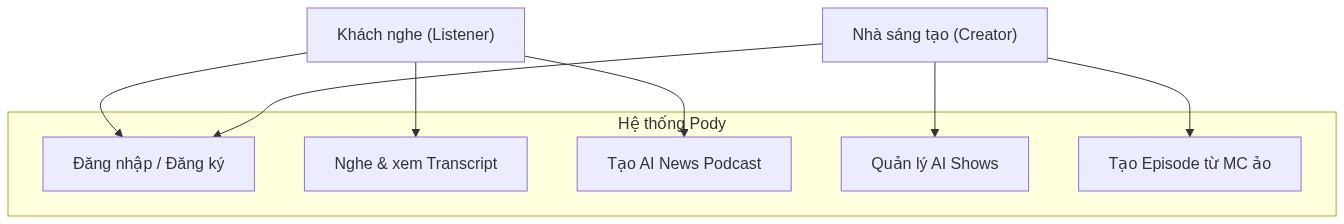
\includegraphics[width=\textwidth]{usecase_overview.png}
%   \caption{Sơ đồ use case tổng quan ứng dụng Pody}
%   \label{fig:usecase-tq}
% \end{figure}

% ---- 2.4 ER tổng quan theo cụm service ----
\section{Mô hình dữ liệu tổng quan (ER theo cụm service)}
\label{sec:er-tong-quan}

Vì mỗi service có database riêng (database-per-service pattern), mô hình ER được trình bày theo từng cụm. Giữa các database không có foreign key vật lý chéo service -- chỉ tham chiếu bằng external ID (ví dụ: \texttt{user\_id}, \texttt{show\_id}, \texttt{article\_id}).

\subsection{Identity DB}

Database của \texttt{identity-service}, quản lý thông tin người dùng và xác thực.

\begin{table}[H]
\centering
\caption{Các bảng trong Identity DB}
\label{tab:er-identity}
\renewcommand{\arraystretch}{1.3}
\small
\begin{tabularx}{\textwidth}{|l|X|}
\hline
\textbf{Bảng} & \textbf{Mô tả} \\
\hline
\texttt{users} & Thông tin người dùng: email, display name, username, avatar, account type, status, locale. \\
\hline
\texttt{user\_identities} & Liên kết tài khoản bên thứ ba (Google, Apple): provider, provider\_user\_id. \\
\hline
\texttt{user\_devices} & Thiết bị người dùng: platform (ios/android/web), push token. \\
\hline
\texttt{auth\_sessions} & Phiên đăng nhập: refresh token hash, thời hạn, trạng thái revoke. \\
\hline
\texttt{email\_verification\_tokens} & Token xác minh email: token hash, thời hạn, trạng thái sử dụng. \\
\hline
\texttt{password\_reset\_tokens} & Token đặt lại mật khẩu: token hash, thời hạn. \\
\hline
\texttt{outbox\_events} & Transactional outbox pattern: event chờ publish lên Kafka. \\
\hline
\texttt{inbox\_processed\_events} & Idempotency: theo dõi event đã xử lý để tránh xử lý trùng. \\
\hline
\end{tabularx}
\end{table}

\subsection{Content DB}

Database của \texttt{content-service}, quản lý nội dung podcast.

\begin{table}[H]
\centering
\caption{Các bảng trong Content DB}
\label{tab:er-content}
\renewcommand{\arraystretch}{1.3}
\small
\begin{tabularx}{\textwidth}{|l|X|}
\hline
\textbf{Bảng} & \textbf{Mô tả} \\
\hline
\texttt{categories} & Danh mục nội dung: slug, name, icon, color, applies\_to (show/news/mixed). \\
\hline
\texttt{tags} & Thẻ gắn: slug, name. \\
\hline
\texttt{shows} & Show podcast: title, slug, content type, language, cover image, publish status, visibility, monetization. \\
\hline
\texttt{show\_categories} & Liên kết show -- category (nhiều-nhiều), có is\_primary. \\
\hline
\texttt{show\_tags} & Liên kết show -- tag (nhiều-nhiều). \\
\hline
\texttt{show\_hosts} & Host của show: display name, avatar, role (host/co\_host/guest/narrator), persona type (human/ai). \\
\hline
\texttt{episodes} & Episode trong show: title, slug, audio URL, duration, publish status, listen/like/comment count. \\
\hline
\texttt{episode\_tags} & Liên kết episode -- tag. \\
\hline
\texttt{episode\_assets} & Tài nguyên đính kèm episode: transcript, waveform, subtitle, cover, attachment. \\
\hline
\texttt{episode\_segments} & Đoạn transcript phân theo speaker: segment index, start/end ms, text content. \\
\hline
\texttt{episode\_bookmarks} & Bookmark episode của user: user\_id + episode\_id. \\
\hline
\texttt{episode\_companion\_blocks} & Nội dung bổ trợ: timeline, quiz, takeaway, flashcards, chapter list. \\
\hline
\end{tabularx}
\end{table}

\subsection{AI DB}

Database của \texttt{ai-service}, quản lý dữ liệu AI và quy trình tạo podcast.

\begin{table}[H]
\centering
\caption{Các bảng trong AI DB}
\label{tab:er-ai}
\renewcommand{\arraystretch}{1.3}
\small
\begin{tabularx}{\textwidth}{|l|X|}
\hline
\textbf{Bảng} & \textbf{Mô tả} \\
\hline
\texttt{voice\_profiles} & Hồ sơ giọng nói: provider (google/openai/elevenlabs), voice ID, gender, language, sample audio. \\
\hline
\texttt{chat\_threads} & Luồng chat với AI: owner user, title, status. \\
\hline
\texttt{chat\_messages} & Tin nhắn trong thread: role (user/assistant/system), text content, plan reference. \\
\hline
\texttt{chat\_attachments} & File đính kèm tin nhắn: image, document, audio. \\
\hline
\texttt{production\_plans} & Kế hoạch sản xuất: series title, description, tone, status, target show. \\
\hline
\texttt{production\_plan\_hosts} & Host trong plan: voice profile, role, persona type. \\
\hline
\texttt{production\_plan\_sources} & Nguồn tham khảo: article ID, title, publisher, URL, summary. \\
\hline
\texttt{production\_plan\_tags} & Thẻ gắn cho plan. \\
\hline
\texttt{production\_plan\_episode\_drafts} & Bản nháp episode: title, description, estimated duration, status. \\
\hline
\texttt{generation\_jobs} & Job tạo nội dung: plan/script/audio/image/transcript/show\_creation/publish, status, input/output payload. \\
\hline
\end{tabularx}
\end{table}

\subsection{Article DB}

Database của \texttt{article\_service}, quản lý bài báo và tương tác.

\begin{table}[H]
\centering
\caption{Các bảng trong Article DB}
\label{tab:er-article}
\renewcommand{\arraystretch}{1.3}
\small
\begin{tabularx}{\textwidth}{|l|X|}
\hline
\textbf{Bảng} & \textbf{Mô tả} \\
\hline
\texttt{news\_sources} & Nguồn tin RSS: domain, name, RSS URL, reliability score, status. \\
\hline
\texttt{articles} & Bài báo: title, author, summary, content, original URL, thumbnail, published\_at. \\
\hline
\texttt{categories} & Danh mục bài báo: slug, name, description. \\
\hline
\texttt{category\_articles} & Liên kết article -- category: assignment source (manual/semantic), is\_primary, score, model. \\
\hline
\texttt{category\_users} & Theo dõi category của user. \\
\hline
\texttt{article\_stats} & Thống kê bài báo: view count. \\
\hline
\texttt{article\_interactions} & Tương tác: user -- article -- interaction type (LIKE, LOVE, ...). \\
\hline
\texttt{article\_comments} & Bình luận bài báo: user, content. \\
\hline
\texttt{article\_metrics} & Metric đọc bài: reading time seconds. \\
\hline
\end{tabularx}
\end{table}

\subsection{Embedding DB}

Database của \texttt{embedding\_service}, lưu trữ vector embedding và kết quả gán category.

\begin{table}[H]
\centering
\caption{Các bảng trong Embedding DB}
\label{tab:er-embedding}
\renewcommand{\arraystretch}{1.3}
\small
\begin{tabularx}{\textwidth}{|l|X|}
\hline
\textbf{Bảng} & \textbf{Mô tả} \\
\hline
\texttt{article\_embedding\_documents} & Document gốc để embedding: article\_id, title, content hash, status. \\
\hline
\texttt{article\_embedding\_chunks} & Chunk text: document reference, chunk index, text content, char range. \\
\hline
\texttt{article\_chunk\_embeddings} & Vector embedding của chunk: embedding vector (pgvector), model, version. \\
\hline
\texttt{article\_document\_embeddings} & Vector embedding tổng hợp của document. \\
\hline
\texttt{category\_embeddings} & Embedding vector cho mỗi category (dùng để gán category ngữ nghĩa). \\
\hline
\texttt{article\_category\_matches} & Kết quả matching article -- category: similarity score, rank. \\
\hline
\texttt{embedding\_jobs} & Job tạo embedding: status, article reference, error tracking. \\
\hline
\end{tabularx}
\end{table}

\subsection{Notification DB}

Database của \texttt{notification-service}, quản lý thông báo và gửi email.

\begin{table}[H]
\centering
\caption{Các bảng trong Notification DB}
\label{tab:er-notification}
\renewcommand{\arraystretch}{1.3}
\small
\begin{tabularx}{\textwidth}{|l|X|}
\hline
\textbf{Bảng} & \textbf{Mô tả} \\
\hline
\texttt{notifications} & Thông báo in-app: user\_id, actor, type, target, title, body, is\_read. \\
\hline
\texttt{user\_notification\_settings} & Cài đặt thông báo: push/email/new episode/comment/follow/marketing enabled. \\
\hline
\texttt{delivery\_logs} & Log gửi thông báo: channel (email/push), status, provider message ID, error. \\
\hline
\texttt{templates} & Template thông báo: code, channel, title/body template. \\
\hline
\texttt{outbox\_events} & Outbox pattern cho event nội bộ. \\
\hline
\texttt{inbox\_processed\_events} & Idempotency: event đã xử lý. \\
\hline
\end{tabularx}
\end{table}

\noindent
\textbf{Lưu ý quan trọng:} Giữa các database không có foreign key vật lý chéo service. Ví dụ, bảng \texttt{notifications} có trường \texttt{user\_id} nhưng đây chỉ là external ID tham chiếu đến \texttt{users.id} trong Identity DB, không phải foreign key constraint.

% Placeholder cho hình ER tổng quan
% \begin{figure}[H]
%   \centering
%   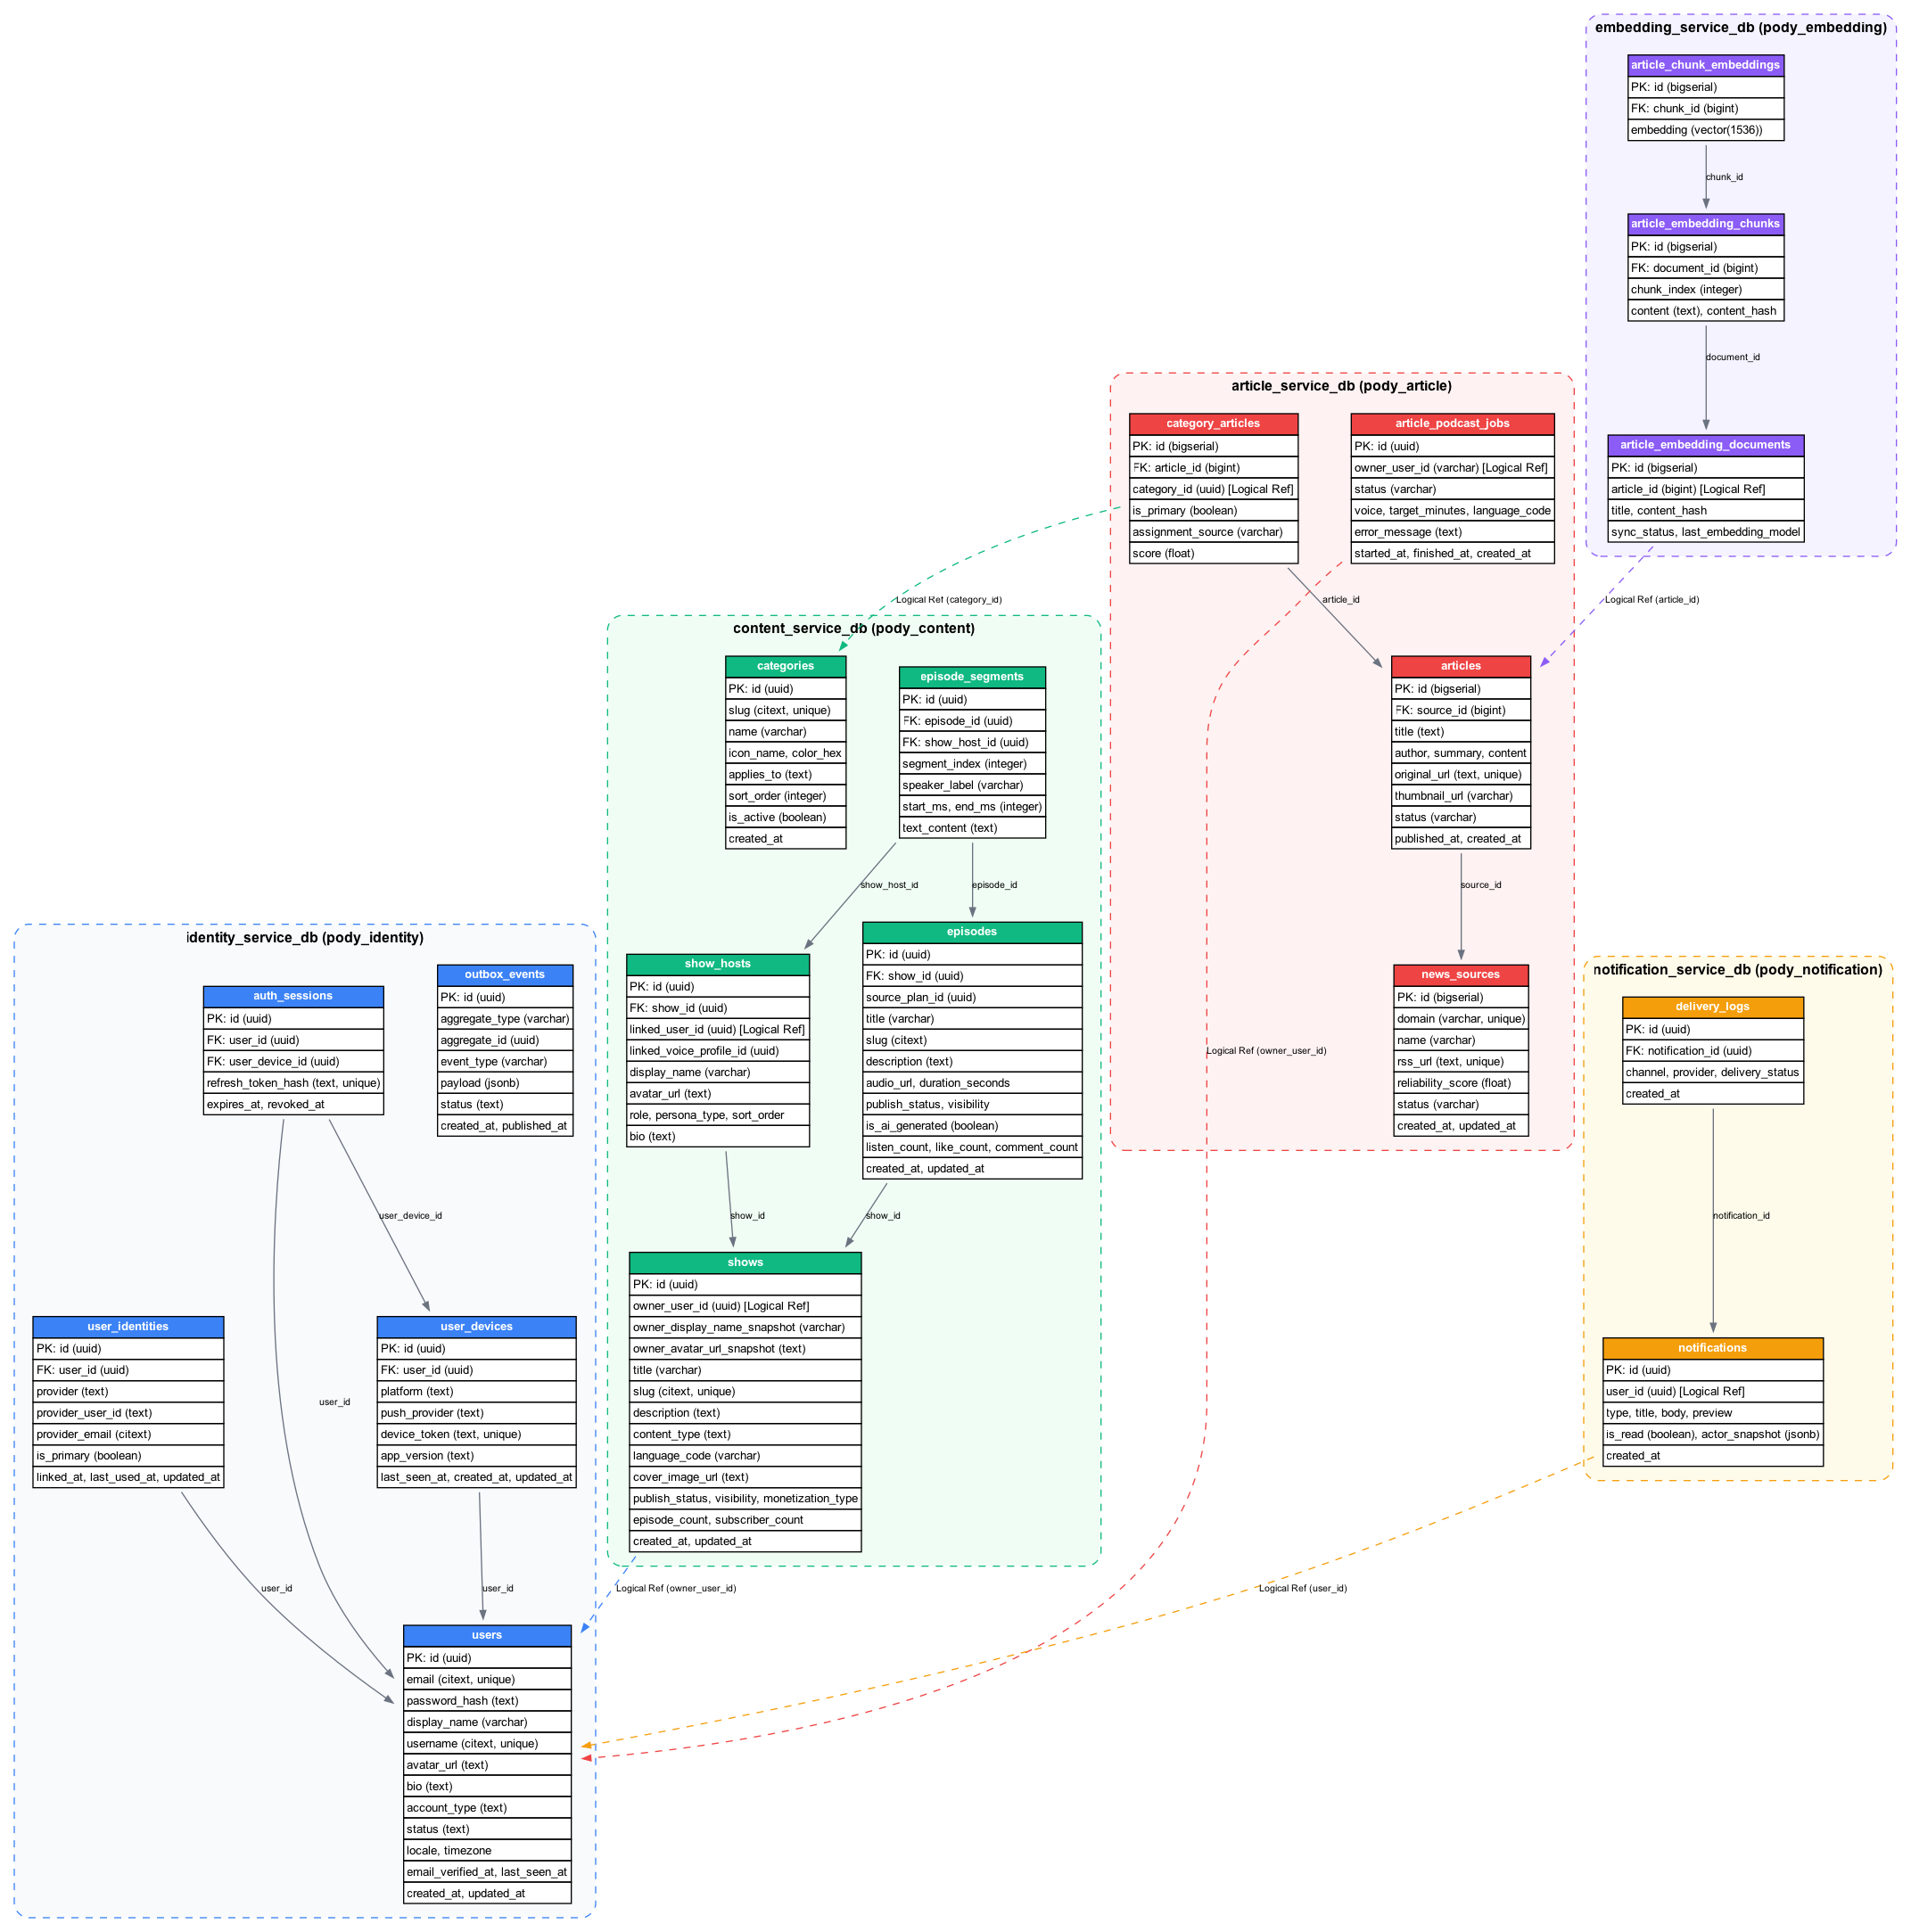
\includegraphics[width=\textwidth]{erd_diagram.png}
%   \caption{Sơ đồ ER tổng quan theo cụm service}
%   \label{fig:er-tq}
% \end{figure}

% ---- 2.5 Mô hình triển khai tổng quát ----
\section{Mô hình triển khai}
\label{sec:trien-khai}

Toàn bộ hệ thống Pody được triển khai trên môi trường local thông qua \textbf{Docker Compose}. Bảng~\ref{tab:deployment} mô tả chi tiết các container và port mapping.

\begin{table}[H]
\centering
\caption{Mô hình triển khai Docker Compose}
\label{tab:deployment}
\renewcommand{\arraystretch}{1.3}
\small
\begin{tabularx}{\textwidth}{|l|c|X|}
\hline
\textbf{Container} & \textbf{Port} & \textbf{Mô tả} \\
\hline
\texttt{api-gateway} & 8080 &
  Cổng vào hệ thống. Reverse proxy, JWT auth, CORS. \\
\hline
\texttt{identity-service} & 8081 &
  Xác thực, user profile, outbox publisher. \\
\hline
\texttt{content-service} & 8082 &
  Show, episode, bookmark, home feed. \\
\hline
\texttt{article-service} & 8084 &
  Bài báo, category, reaction, comment, crawler, podcast job. \\
\hline
\texttt{ai-service} & 8085 &
  Chat-create, production plan, generation jobs, TTS. \\
\hline
\texttt{notification-service} & 8087 &
  Notification inbox, email sender, Kafka consumer. \\
\hline
\texttt{embedding-service} & 8088 &
  Embedding, semantic search, category matching. \\
\hline
\texttt{article-postgres} & 5433 &
  PostgreSQL cho Article Service (WAL logical cho CDC). \\
\hline
\texttt{embedding-postgres} & 5434 &
  PostgreSQL + pgvector cho Embedding Service. \\
\hline
\texttt{migrations} & -- &
  Init-container: chạy migration cho Identity, Content, AI, Notification DB. \\
\hline
\texttt{kafka} & 9092 &
  Apache Kafka 4.0 (KRaft mode, không cần Zookeeper). \\
\hline
\texttt{debezium-connect} & 8083 &
  Debezium CDC connector cho Article DB. \\
\hline
\texttt{kafka-ui} & 8090 &
  Giao diện web quản lý Kafka. \\
\hline
\texttt{redis} & 6379 &
  Redis 7 Alpine -- cache phụ trợ. \\
\hline
\texttt{minio} & 9000/9001 &
  Object storage (S3-compatible). Port 9001 cho MinIO Console. \\
\hline
\end{tabularx}
\end{table}

\subsection{Thứ tự khởi động}

Docker Compose quản lý thứ tự khởi động thông qua \texttt{depends\_on} với health check:

\begin{enumerate}[leftmargin=2cm]
  \item \textbf{Infrastructure:} Kafka, Redis, MinIO, PostgreSQL instances khởi động trước.
  \item \textbf{Database init:} \texttt{migrations} (Identity/Content/AI/Notification DB) và \texttt{article-db-init}, \texttt{embedding-db-init} chạy migration/seed.
  \item \textbf{CDC:} Debezium Connect khởi động sau Kafka và Article Postgres. \texttt{debezium-register} đăng ký connector.
  \item \textbf{Backend services:} Các service khởi động sau khi database sẵn sàng, mỗi service expose health check endpoint \texttt{/healthz}.
  \item \textbf{API Gateway:} Khởi động cuối cùng, sau khi tất cả backend service healthy.
\end{enumerate}

\subsection{Kiểm tra hệ thống}

Sau khi hệ thống khởi động, có thể kiểm tra qua các URL:

\begin{itemize}[leftmargin=2cm]
  \item Health check: \texttt{http://localhost:8080/healthz}
  \item Tổng hợp docs: \texttt{http://localhost:8080/docs}
  \item Route metadata: \texttt{http://localhost:8080/api/v1/\_meta/routes}
  \item Identity docs: \texttt{http://localhost:8080/api/v1/public/identity/docs}
  \item Content docs: \texttt{http://localhost:8080/api/v1/public/content/docs}
  \item AI docs: \texttt{http://localhost:8080/api/v1/public/ai/docs}
  \item Notification docs: \texttt{http://localhost:8080/api/v1/public/notifications/docs}
  \item Kafka UI: \texttt{http://localhost:8090}
  \item MinIO Console: \texttt{http://localhost:9001}
\end{itemize}

% ---- 2.6 Bảng mapping tổng hợp ----
\section{Bảng mapping Service -- Chức năng -- Database -- Endpoint chính}
\label{sec:mapping}

\begin{table}[H]
\centering
\caption{Mapping tổng hợp service}
\label{tab:mapping}
\renewcommand{\arraystretch}{1.3}
\scriptsize
\begin{tabularx}{\textwidth}{|l|l|l|X|}
\hline
\textbf{Service} & \textbf{Database} & \textbf{Chức năng chính} & \textbf{Endpoint tiêu biểu} \\
\hline
identity & Identity DB &
  Auth, profile, outbox &
  \texttt{POST /public/identity/sign-up}, \texttt{sign-in}, \texttt{google}, \texttt{refresh}, \texttt{GET /identity/me} \\
\hline
content & Content DB &
  Show, episode, bookmark &
  \texttt{GET /public/content/home}, \texttt{shows/\{id\}}, \texttt{episodes/\{id\}}, \texttt{POST /content/bookmarks} \\
\hline
ai & AI DB &
  Chat, plan, jobs &
  \texttt{POST /ai/chat-create/threads}, \texttt{threads/\{id\}/messages}, \texttt{POST /ai/plans/\{id\}/create-show} \\
\hline
article & Article DB &
  Báo, category, podcast &
  \texttt{GET /article}, \texttt{/article/\{id\}}, \texttt{POST /article/\{id\}/reactions}, \texttt{POST /article/podcast-jobs} \\
\hline
embedding & Embedding DB &
  Embedding, search &
  \texttt{POST /public/embedding/articles/search} \\
\hline
notification & Notification DB &
  Thông báo, email &
  \texttt{GET /notifications}, \texttt{/unread-count}, \texttt{PATCH /\{id\}/read}, \texttt{PUT /settings} \\
\hline
\end{tabularx}
\end{table}

\clearpage

% ============================================================
% CHƯƠNG 3 - THIẾT KẾ CHI TIẾT CÁ NHÂN
% ============================================================
\chapter{THIẾT KẾ CHI TIẾT CÁ NHÂN}
\label{chap:thiet-ke-chi-tiet}

Chương này trình bày phần thiết kế chi tiết theo phạm vi phụ trách của từng thành viên. Mỗi tiểu mục bám theo cùng một cấu trúc: phạm vi service, chức năng chính, use case chi tiết, mô hình component, mô hình dữ liệu, sequence diagram, API contract, giao diện liên quan, kết quả đạt được và hạn chế.

\section{Lê Minh Ngọc -- Thông báo: \texttt{notification-service}}
\label{sec:phase3-notification}

\subsection{Phạm vi phụ trách}

Lê Minh Ngọc phụ trách notification inbox, unread count, mark read/read all, notification settings, internal API tạo notification, gửi email xác minh/reset password, consume Kafka event, retry/DLQ, processed-event tracking và delivery logs.

\subsection{Use case chi tiết}

\begin{table}[H]
\centering
\caption{Use case chi tiết Notification Service}
\label{tab:uc-notification}
\renewcommand{\arraystretch}{1.3}
\small
\begin{tabularx}{\textwidth}{|c|l|l|X|}
\hline
\textbf{Mã} & \textbf{Use case} & \textbf{Tác nhân} & \textbf{Mô tả} \\
\hline
NO-UC-01 & Xem danh sách thông báo & User & Lấy notification inbox theo user, hỗ trợ phân trang. \\
\hline
NO-UC-02 & Xem unread count & User & Đếm số thông báo chưa đọc để hiển thị badge. \\
\hline
NO-UC-03 & Đánh dấu đã đọc & User & Cập nhật \texttt{read\_at} cho một notification. \\
\hline
NO-UC-04 & Đánh dấu tất cả đã đọc & User & Cập nhật toàn bộ notification chưa đọc của user. \\
\hline
NO-UC-05 & Cập nhật settings & User & Bật/tắt email, push hoặc nhóm notification theo nhu cầu. \\
\hline
NO-UC-06 & Gửi email verification/reset & Hệ thống & Consume Kafka event từ Identity, gửi email và ghi delivery log. \\
\hline
NO-UC-07 & Tạo notification nội bộ & Internal service & AI Service hoặc service khác gọi internal API để tạo in-app notification. \\
\hline
\end{tabularx}
\end{table}

\subsection{Component diagram}

\begin{figure}[H]
  \centering
  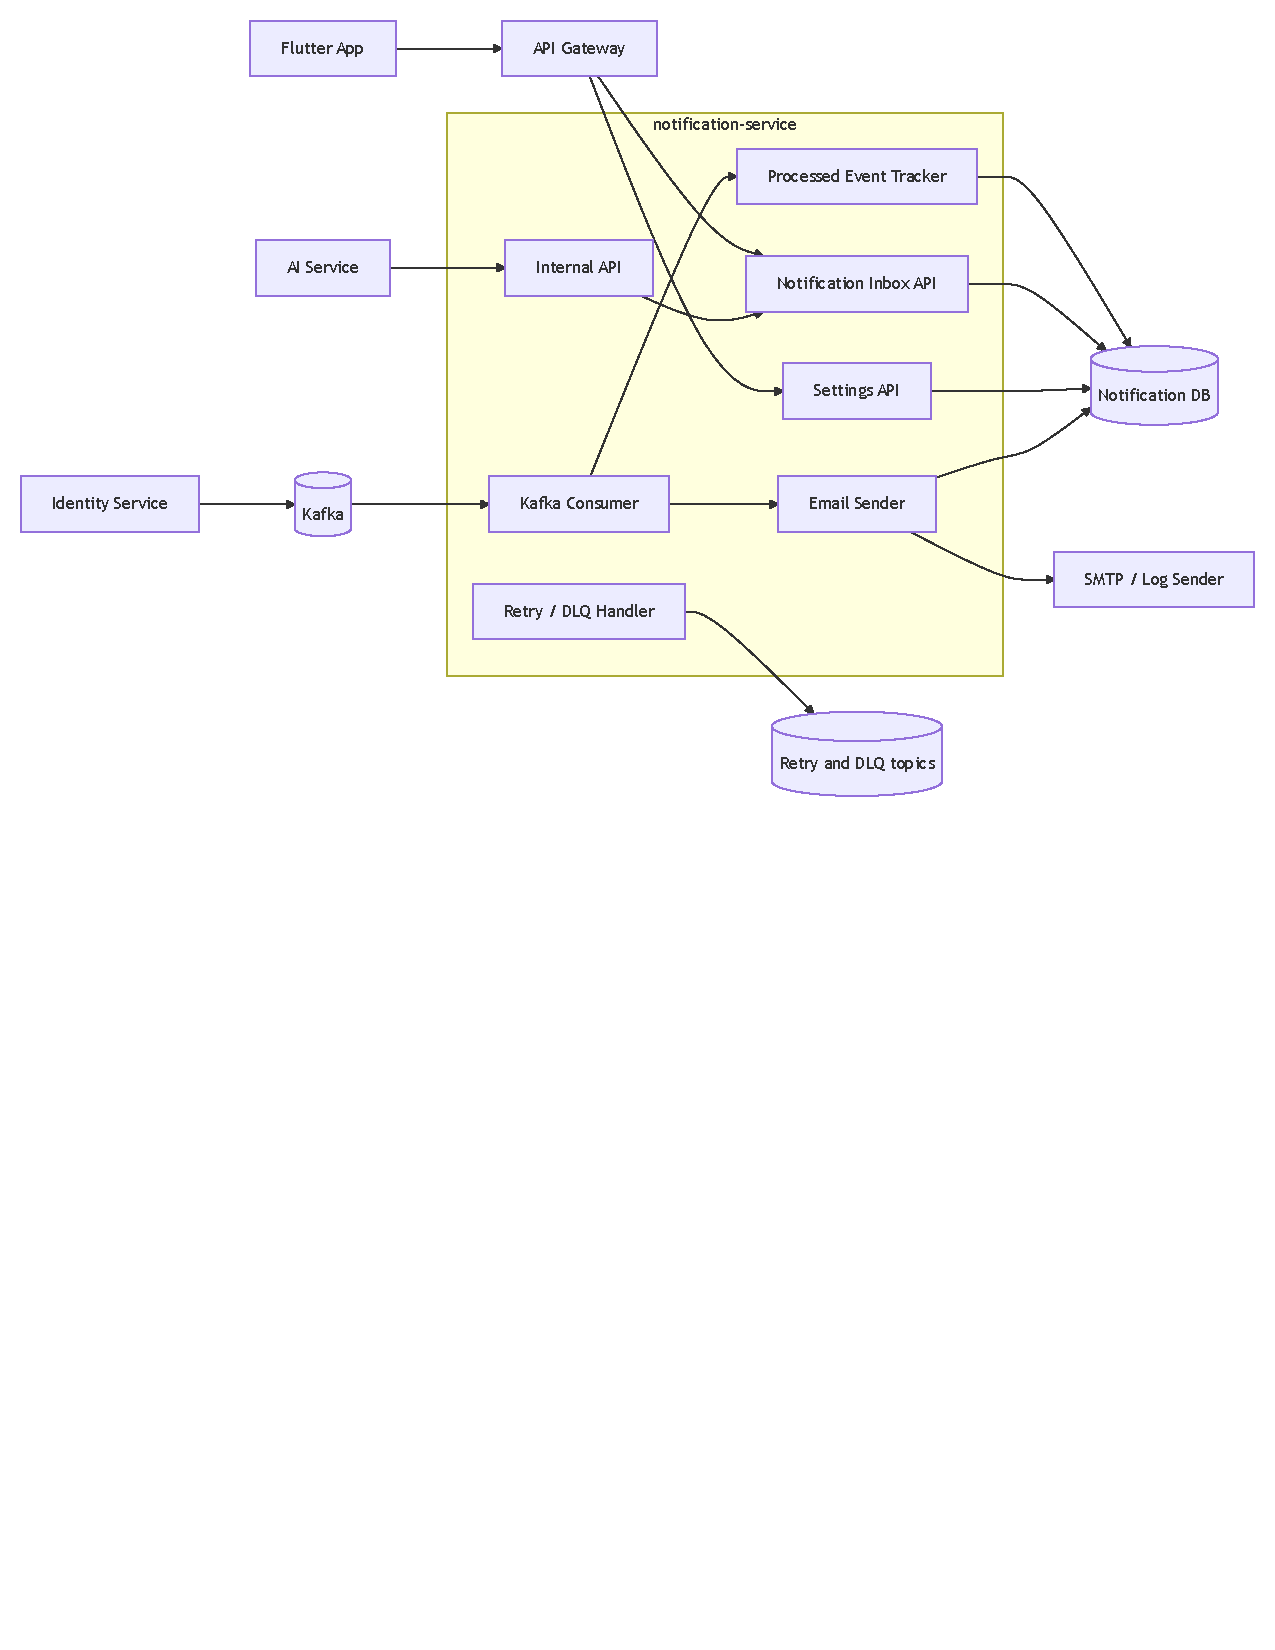
\includegraphics[width=\textwidth,height=0.78\textheight,keepaspectratio]{diagrams/component_notification.pdf}
  \caption{Component diagram \texttt{notification-service}}
  \label{fig:component-notification}
\end{figure}

\subsection{Mô hình dữ liệu riêng}

Notification DB gồm \texttt{notifications}, \texttt{user\_notification\_settings}, \texttt{delivery\_logs}, \texttt{templates} và \texttt{inbox\_processed\_events}. Trường \texttt{user\_id} là external ID từ Identity DB, không phải foreign key vật lý. Bảng processed event giúp idempotency khi consume Kafka để tránh gửi email hoặc tạo notification trùng.

\begin{figure}[H]
  \centering
  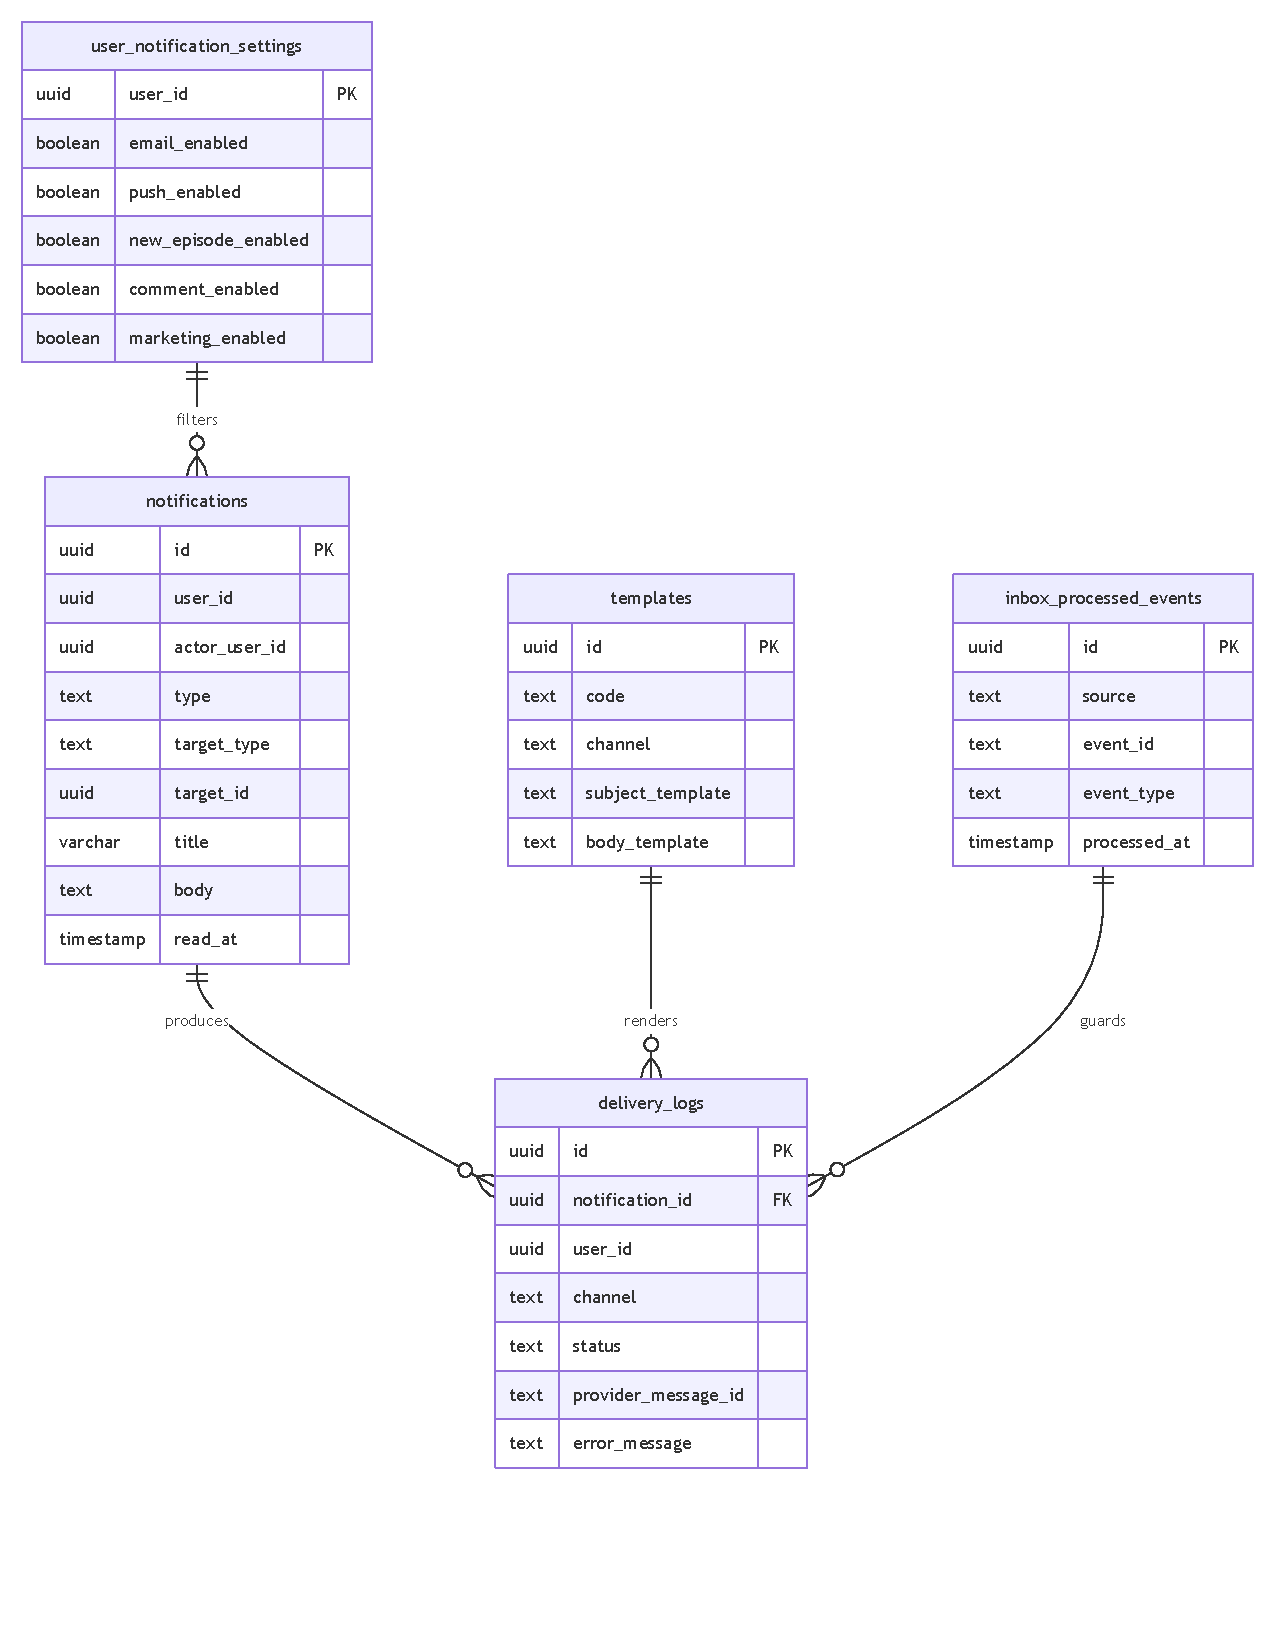
\includegraphics[width=\textwidth,height=0.78\textheight,keepaspectratio]{diagrams/er_notification.pdf}
  \caption{ER riêng cho Notification DB}
  \label{fig:er-notification-detail}
\end{figure}

\subsection{Sequence diagram}

\begin{figure}[H]
  \centering
  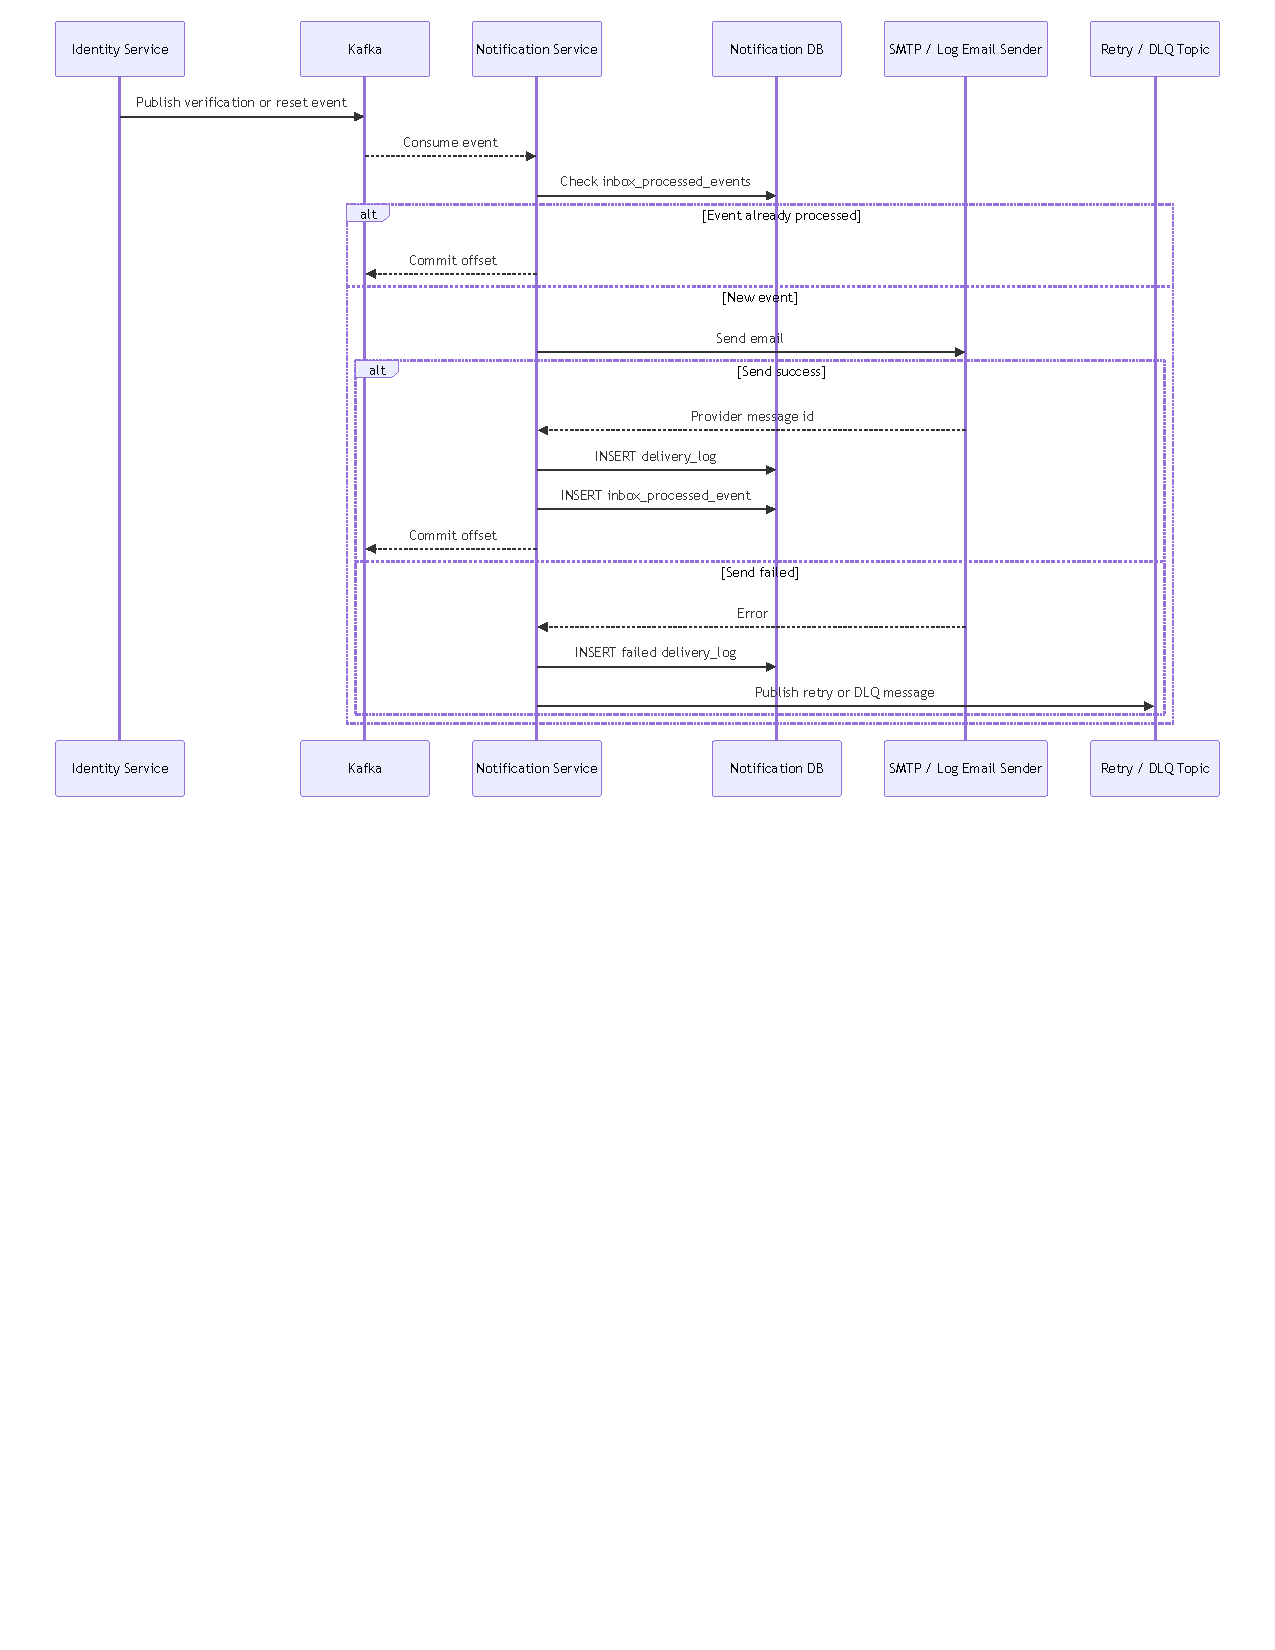
\includegraphics[width=\textwidth,height=0.78\textheight,keepaspectratio]{diagrams/seq_notification_email.pdf}
  \caption{Sequence diagram gửi email verification/reset password}
  \label{fig:seq-notification-email}
\end{figure}

\begin{figure}[H]
  \centering
  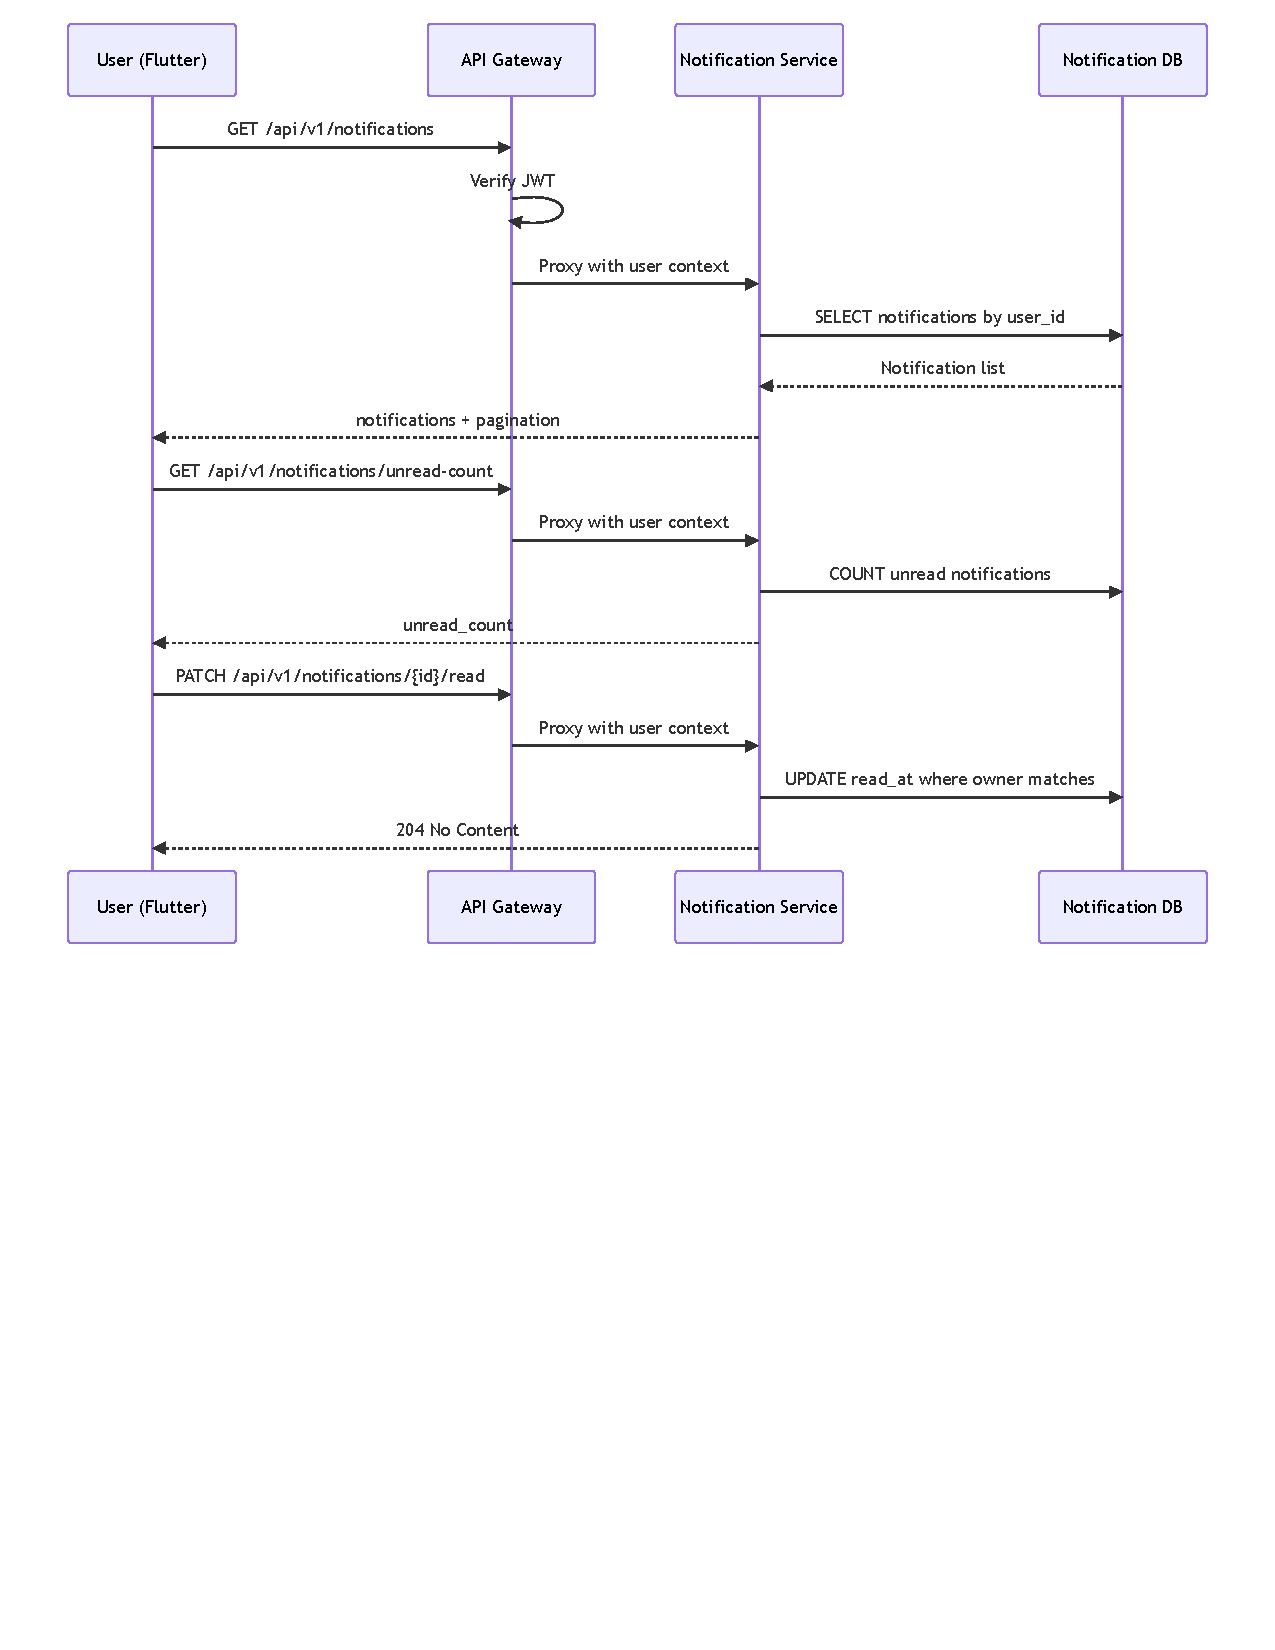
\includegraphics[width=\textwidth,height=0.78\textheight,keepaspectratio]{diagrams/seq_notification_inbox.pdf}
  \caption{Sequence diagram xem và đánh dấu thông báo}
  \label{fig:seq-notification-inbox}
\end{figure}

\subsection{API/service contract}

\begin{table}[H]
\centering
\caption{Endpoint chính Notification Service}
\label{tab:endpoint-notification}
\renewcommand{\arraystretch}{1.3}
\scriptsize
\begin{tabularx}{\textwidth}{|l|l|X|}
\hline
\textbf{Method} & \textbf{Endpoint} & \textbf{Mục đích} \\
\hline
GET & \texttt{/api/v1/notifications} & Lấy danh sách notification của user. \\
\hline
GET & \texttt{/api/v1/notifications/unread-count} & Lấy số notification chưa đọc. \\
\hline
PATCH & \texttt{/api/v1/notifications/\{id\}/read} & Đánh dấu một notification đã đọc. \\
\hline
PATCH & \texttt{/api/v1/notifications/read-all} & Đánh dấu tất cả notification đã đọc. \\
\hline
GET & \texttt{/api/v1/notifications/settings} & Lấy cài đặt thông báo. \\
\hline
PUT & \texttt{/api/v1/notifications/settings} & Cập nhật cài đặt thông báo. \\
\hline
POST & \texttt{/internal/notifications/email/verification} & Internal endpoint gửi email verification nếu cần gọi trực tiếp. \\
\hline
POST & \texttt{/internal/notifications/inbox} & Internal endpoint tạo in-app notification. \\
\hline
\end{tabularx}
\end{table}

\subsection{Giao diện liên quan và kết quả đạt được}

Các giao diện liên quan gồm notifications tab/list, badge unread count, notification settings và log email verification/reset password trong môi trường local. Service đã hỗ trợ cả notification chủ động qua internal API và notification/email phát sinh từ event bất đồng bộ.

\subsection{Hạn chế riêng}

Ở phạm vi bài tập lớn, email sender có thể dùng log/smtp local nên chưa phản ánh đầy đủ deliverability thực tế. Push notification mobile, template management nâng cao và dashboard theo dõi retry/DLQ là các phần có thể phát triển tiếp.


\section{Tổng hợp đầu ra Phase 3}
\label{sec:phase3-summary}

Bảng~\ref{tab:phase3-output} tổng hợp đầu ra của phần cá nhân trong Chương 3.

\begin{table}[H]
\centering
\caption{Tổng hợp đầu ra Phase 3 -- Notification}
\label{tab:phase3-output}
\renewcommand{\arraystretch}{1.3}
\scriptsize
\begin{tabularx}{\textwidth}{|l|X|X|}
\hline
\textbf{Cụm phụ trách} & \textbf{Sơ đồ đã bổ sung} & \textbf{Nội dung chính} \\
\hline
Notification & Component, ER, sequence email event, sequence inbox/read & Inbox, unread count, settings, internal notification, email delivery, idempotency, retry/DLQ. \\
\hline
\end{tabularx}
\end{table}

\vspace{1cm}
\noindent\rule{\textwidth}{0.4pt}

\noindent
\textit{Kết thúc Phase 3 -- Thiết kế chi tiết cá nhân.}

\clearpage

% ============================================================
% CHƯƠNG 4 - KẾT QUẢ, THỬ NGHIỆM VÀ ĐÁNH GIÁ
% ============================================================
\chapter{KẾT QUẢ, THỬ NGHIỆM VÀ ĐÁNH GIÁ}
\label{chap:ket-qua}

Chương này tách rõ kết quả chung của nhóm và kết quả riêng của phần cá nhân: Lê Minh Ngọc -- Thông báo. Phần triển khai local được giữ ở mức tổng quát, còn bảng kết quả, kiểm thử và số liệu minh chứng tập trung vào cụm Notification.

\section{Kết quả ứng dụng}
\label{sec:ket-qua-ung-dung}

\subsection{Kết quả tổng quát cấp nhóm}

Hệ thống đã được tổ chức theo kiến trúc microservices với Flutter App, API Gateway và các backend service độc lập. Các service chính có health check, tài liệu OpenAPI/Swagger, database riêng và có thể chạy local thông qua Docker Compose.

\begin{table}[H]
\centering
\caption{Kết quả tổng quát cấp nhóm}
\label{tab:ket-qua-tong-quat}
\renewcommand{\arraystretch}{1.3}
\small
\begin{tabularx}{\textwidth}{|l|X|c|}
\hline
\textbf{Hạng mục} & \textbf{Kết quả đạt được} & \textbf{Trạng thái} \\
\hline
Mobile app & Flutter App có các màn hình auth, home/show/episode, news/article, create AI, profile và notifications. & Đạt \\
\hline
API Gateway & Điều phối request, tách route public/protected, kiểm tra JWT và proxy đến service đích. & Đạt \\
\hline
Backend services & Identity, Content, AI, Article, Embedding và Notification được tách theo nghiệp vụ. & Đạt \\
\hline
Database-per-service & Mỗi service có schema/database riêng, tham chiếu chéo qua external ID thay vì foreign key vật lý. & Đạt \\
\hline
Event-driven & Kafka/Debezium hỗ trợ outbox email, CDC bài báo, category sync và xử lý bất đồng bộ. & Đạt \\
\hline
Local deployment & Docker Compose khởi động infrastructure, database init, services, gateway, Kafka UI, Redis và MinIO. & Đạt \\
\hline
\end{tabularx}
\end{table}

\subsection{Kết quả theo phạm vi cá nhân}

\begin{table}[H]
\centering
\caption{Kết quả cá nhân -- Notification}
\label{tab:ket-qua-ca-nhan}
\renewcommand{\arraystretch}{1.3}
\small
\begin{tabularx}{\textwidth}{|l|X|}
\hline
\textbf{Nội dung} & \textbf{Kết quả} \\
\hline
Cụm phụ trách & Notification \\
\hline
Chức năng đã hoàn thành & Notification inbox, unread count, mark read/read all, settings, email verification/reset, internal notification, processed-event tracking và retry/DLQ contract. \\
\hline
Minh chứng chính & Notification DB, delivery log, Kafka consumer, internal notification API, màn hình notifications/settings. \\
\hline
\end{tabularx}
\end{table}

\section{Cài đặt và triển khai ứng dụng}
\label{sec:cai-dat-trien-khai}

\subsection{Yêu cầu môi trường}

\begin{itemize}[leftmargin=2cm]
  \item Docker và Docker Compose.
  \item Flutter SDK để chạy mobile app.
  \item File cấu hình môi trường cho các API key nếu chạy đầy đủ luồng AI/TTS/embedding.
  \item Port local chưa bị chiếm: 8080, 8081, 8082, 8083, 8084, 8085, 8087, 8088, 5433, 5434, 6379, 8090, 9000 và 9001.
\end{itemize}

\subsection{Các bước triển khai local}

\begin{enumerate}[leftmargin=2cm]
  \item Kiểm tra Docker Desktop đã chạy.
  \item Cấu hình biến môi trường cần thiết cho Gemini/GenAI, MinIO/GCS hoặc SMTP nếu muốn chạy đầy đủ tính năng bên thứ ba.
  \item Khởi động toàn bộ hệ thống backend bằng Docker Compose.
  \item Chờ các database init/migration hoàn tất và các service chuyển sang trạng thái healthy.
  \item Đăng ký Debezium connector nếu connector chưa được đăng ký tự động.
  \item Chạy Flutter App và trỏ base URL về API Gateway \texttt{http://localhost:8080}.
  \item Kiểm tra health check, docs và các luồng demo chính.
\end{enumerate}

\begin{lstlisting}[language=bash,caption={Lệnh chạy hệ thống local},label={lst:docker-compose-up}]
docker compose up --build
\end{lstlisting}

\subsection{URL kiểm tra nhanh}

\begin{table}[H]
\centering
\caption{URL kiểm tra hệ thống sau khi khởi động}
\label{tab:url-kiem-tra}
\renewcommand{\arraystretch}{1.3}
\small
\begin{tabularx}{\textwidth}{|l|X|}
\hline
\textbf{Mục đích} & \textbf{URL} \\
\hline
Health check Gateway & \texttt{http://localhost:8080/healthz} \\
\hline
Tổng hợp docs & \texttt{http://localhost:8080/docs} \\
\hline
Route metadata & \texttt{http://localhost:8080/api/v1/\_meta/routes} \\
\hline
Kafka UI & \texttt{http://localhost:8090} \\
\hline
MinIO Console & \texttt{http://localhost:9001} \\
\hline
\end{tabularx}
\end{table}

\section{Kết quả thử nghiệm cá nhân}
\label{sec:ket-qua-thu-nghiem}

\begin{longtable}{|p{2.8cm}|p{4.0cm}|p{4.3cm}|p{3.0cm}|p{1.6cm}|}
\caption{Bảng test case cá nhân -- Notification}
\label{tab:test-case}\\
\hline
\textbf{Nhóm chức năng} & \textbf{Test case} & \textbf{Kết quả mong đợi} & \textbf{Kết quả thực tế} & \textbf{TT} \\
\hline
\endfirsthead
\hline
\textbf{Nhóm chức năng} & \textbf{Test case} & \textbf{Kết quả mong đợi} & \textbf{Kết quả thực tế} & \textbf{TT} \\
\hline
\endhead
Notification & Xem danh sách thông báo & Trả notification inbox theo user. & API trả danh sách có phân trang. & Pass \\
\hline
Notification & Xem unread count & Trả số notification chưa đọc. & API trả count theo user. & Pass \\
\hline
Notification & Mark read & Cập nhật trạng thái đã đọc. & \texttt{read\_at}/is\_read được cập nhật. & Pass \\
\hline
Notification & Cập nhật settings & Lưu cấu hình email/push/category notification. & Settings được đọc/ghi qua Notification Service. & Pass \\
\hline
Email event & Gửi email verification/reset & Consume Kafka event, kiểm tra idempotency và ghi delivery log. & Hoạt động khi Kafka/email sender sẵn sàng. & Pass có điều kiện \\
\hline
\end{longtable}

\section{Số liệu minh chứng trong CSDL}
\label{sec:so-lieu-minh-chung}

\begin{table}[H]
\centering
\caption{Số liệu demo cá nhân -- Notification}
\label{tab:so-lieu-demo}
\renewcommand{\arraystretch}{1.3}
\small
\begin{tabularx}{\textwidth}{|l|c|X|}
\hline
\textbf{Hạng mục} & \textbf{Số lượng demo} & \textbf{Nguồn/ghi chú} \\
\hline
Notifications & Chốt khi demo & Phát sinh từ seed inbox hoặc internal notification API. \\
\hline
Unread/read notifications & Chốt khi demo & Đếm theo trạng thái read/unread của user. \\
\hline
Notification settings & Chốt khi demo & Một bản settings theo user khi người dùng cập nhật. \\
\hline
Delivery logs & Chốt khi demo & Phát sinh khi gửi email verification/reset. \\
\hline
Processed events & Chốt khi demo & Theo dõi event đã xử lý để chống trùng. \\
\hline
Retry/DLQ records & Chốt khi demo & Phát sinh khi giả lập lỗi gửi email hoặc lỗi xử lý event. \\
\hline
\end{tabularx}
\end{table}

\section{Đánh giá hạn chế}
\label{sec:han-che}

\subsection{Hạn chế chung}

\begin{itemize}[leftmargin=2cm]
  \item Hệ thống hiện tối ưu cho demo/local, chưa hoàn thiện toàn bộ tiêu chuẩn production như autoscaling, backup, monitoring và alerting.
  \item Database-per-service giúp tách service rõ ràng nhưng đòi hỏi quản lý consistency bằng event, idempotency và retry/DLQ cẩn thận.
\end{itemize}

\subsection{Hạn chế riêng của phần cá nhân}

\begin{itemize}[leftmargin=2cm]
  \item Email sender local/log chưa phản ánh đầy đủ deliverability thực tế.
  \item Push notification mobile, template management nâng cao và dashboard DLQ chưa hoàn thiện.
  \item Cần bổ sung quan sát delivery, retry và alerting nếu triển khai production.
\end{itemize}

\section{Định hướng phát triển}
\label{sec:dinh-huong}

\begin{enumerate}[leftmargin=2cm]
  \item Hoàn thiện recommendation cá nhân hóa dựa trên lịch sử nghe/đọc, favorite categories và embedding similarity.
  \item Bổ sung dashboard quản trị nội dung, nguồn tin, moderation comment và theo dõi chất lượng podcast tạo bằng AI.
  \item Cải thiện AI pipeline với prompt versioning, evaluation, cache kết quả, multi-voice dialogue và kiểm duyệt nội dung tự động.
  \item Triển khai production trên cloud với CI/CD, observability, log aggregation, backup database và secrets management.
  \item Mở rộng notification sang push notification thực tế trên iOS/Android và template management cho nhiều loại email/in-app message.
\end{enumerate}

\section{Tài liệu tham khảo}
\label{sec:tai-lieu-tham-khao}

\begin{enumerate}[leftmargin=2cm]
  \item Flutter documentation: \texttt{https://docs.flutter.dev}
  \item Go documentation: \texttt{https://go.dev/doc}
  \item FastAPI documentation: \texttt{https://fastapi.tiangolo.com}
  \item PostgreSQL documentation: \texttt{https://www.postgresql.org/docs}
  \item pgvector documentation: \texttt{https://github.com/pgvector/pgvector}
  \item Apache Kafka documentation: \texttt{https://kafka.apache.org/documentation}
  \item Debezium documentation: \texttt{https://debezium.io/documentation}
  \item Docker Compose documentation: \texttt{https://docs.docker.com/compose}
  \item Google GenAI/Gemini documentation.
  \item Tài liệu nội bộ repository: README của từng service trong hệ thống Pody.
\end{enumerate}

\vspace{1cm}
\noindent\rule{\textwidth}{0.4pt}

\noindent
\textit{Kết thúc bản báo cáo cá nhân -- Lê Minh Ngọc -- Thông báo.}

\end{document}
